\chapter{Exploration Data Layers}\label{app:A_data_layers}

This appendix steps through each of the data layers (or ``features'') used as predictor and response variables for the machine learning approach to exploration risk mitigation described in Chapters \ref{ch3:expl_ml_prep} and \ref{ch5:ml_results}. For each feature, the source of the data, specific conditioning steps applied to the data, and an image of the final feature map are provided. Refer to Chapter \ref{ch3:expl_ml_prep} for details on methods and routines mentioned by name in the descriptions below.
\vfill
\pagebreak

\section{Average Air Temperature}\label{app:dl_air_temp}
The University of Oregon PRISM Climate Group maintains regularly-updated spatial data sets of climate-related observations, including 30-year normals describing average annual conditions \citep{daly_physiographically_2008, prism_prism_2021}. The 800 m resolution average air temperature grid was downloaded and imported into ArcGIS, then cropped using the Regional Polygon (Figure \ref{fig:feat_airtemp}). This layer required no further processing.

\begin{figure}[H]
\centering
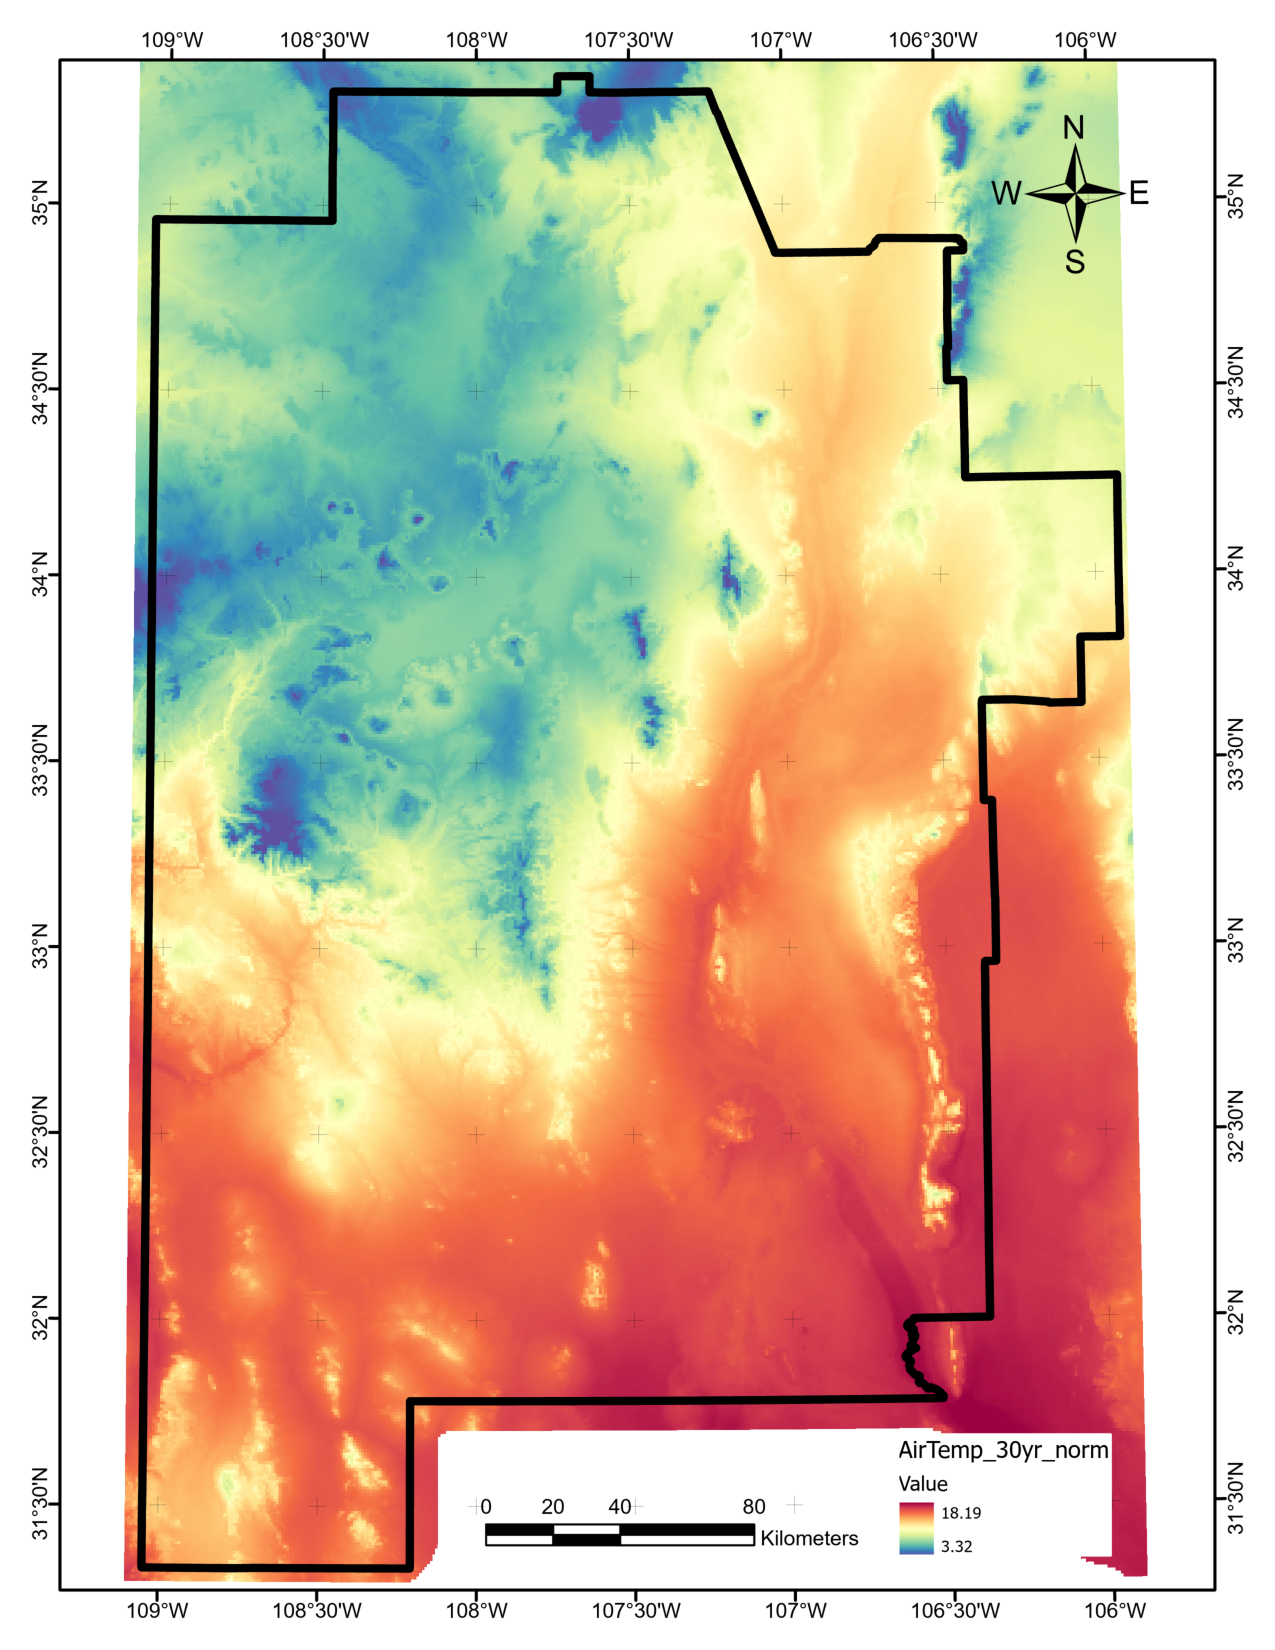
\includegraphics[width=0.75\linewidth]{templates/images/Figure-AvgAirTemp.pdf}
\caption[Average air temperature data layer]{Average air temperature data layer. Units are in $^\circ$C. Data were retrieved from the PRISM website \protect\citep{prism_prism_2021}.}
\label{fig:feat_airtemp}
\end{figure}
\pagebreak

\section{Average Precipitation}\label{app:dl_precip}
The University of Oregon PRISM Climate Group also compiles 30-year normals for precipitation \citep{daly_physiographically_2008, prism_prism_2021}. The 800 m resolution average precipitation grid was downloaded and imported into ArcGIS, then cropped to the Regional Polygon boundary (Figure \ref{fig:feat_precip}). This layer required no further processing.

\begin{figure}[H]
\centering
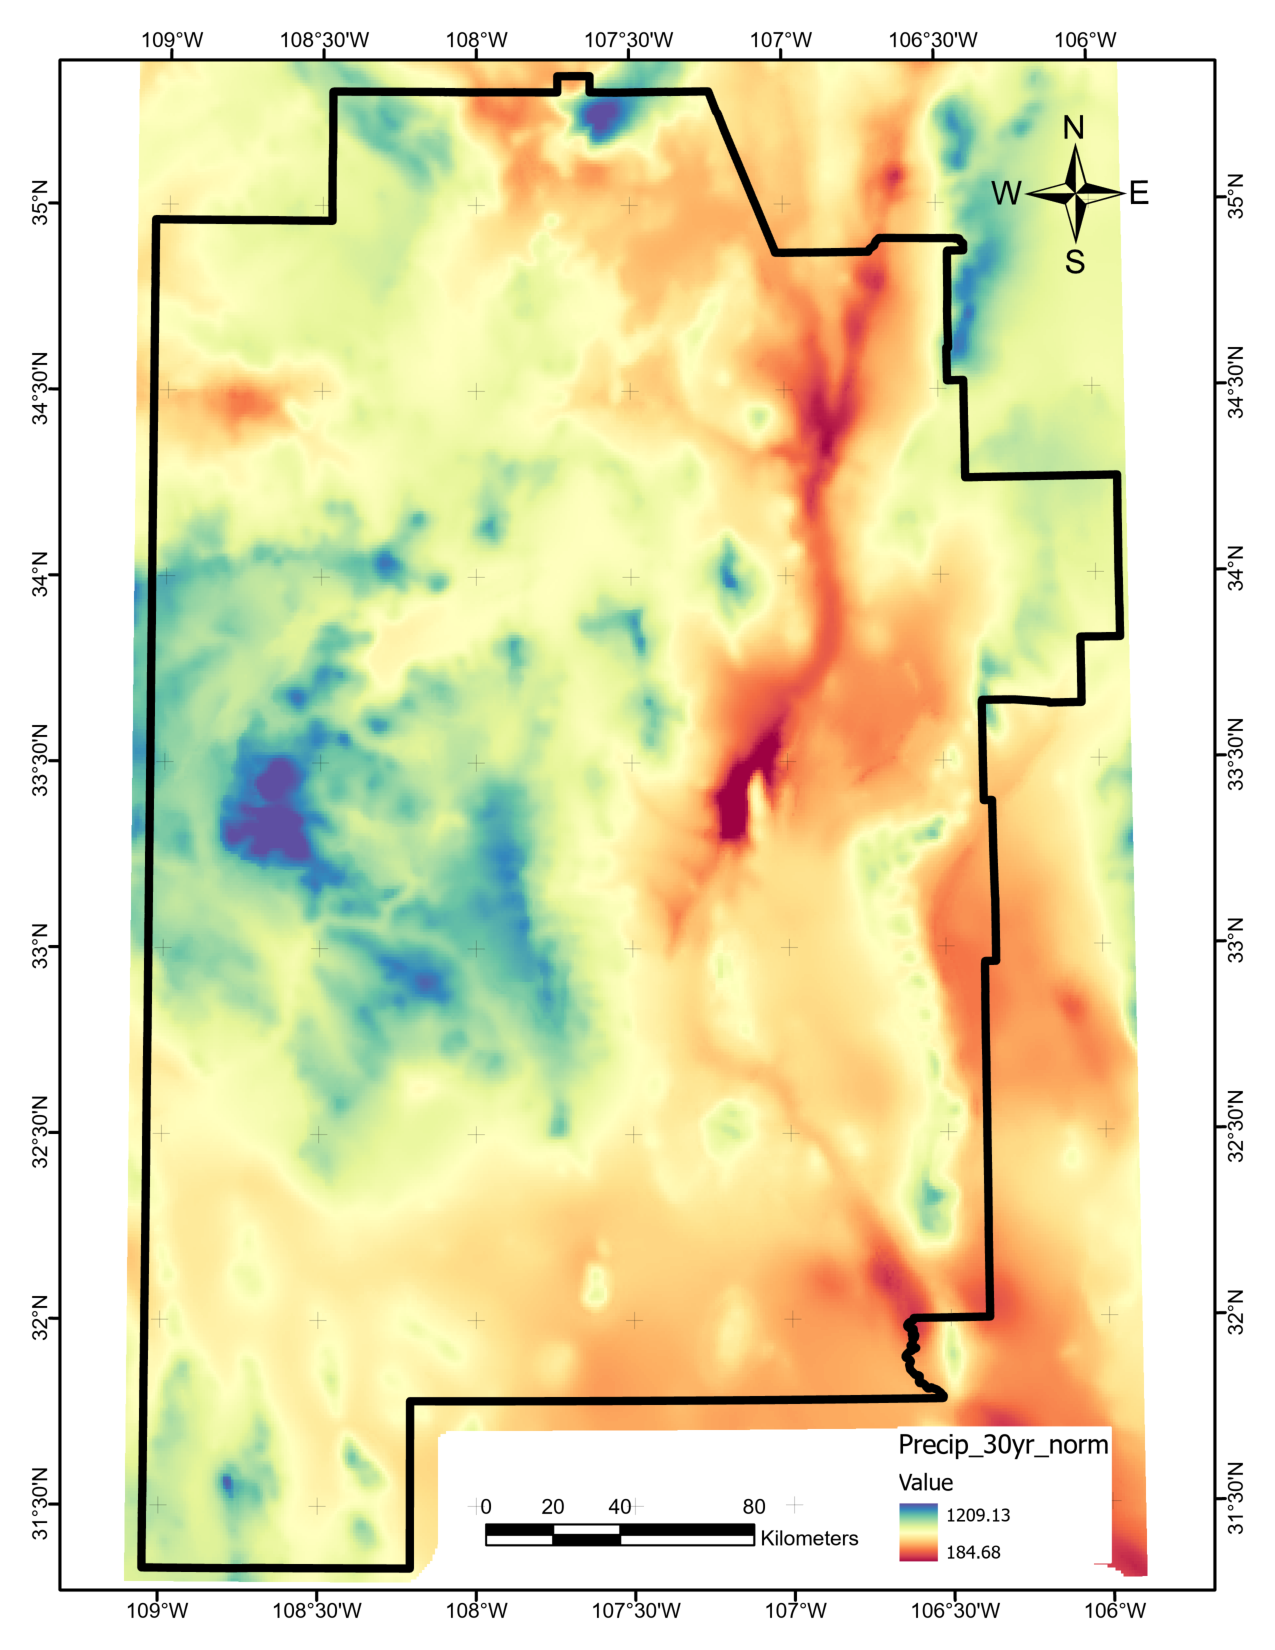
\includegraphics[width=0.75\linewidth]{templates/images/Figure-AvgPrecip.pdf}
\caption[Average precipitation data layer]{Average precipitation data layer. Units are in millimeters. Data were retrieved from the PRISM website \protect\citep{prism_prism_2021}.}
\label{fig:feat_precip}
\end{figure}
\pagebreak

\section{Basement Depth}\label{app:dl_basement_depth}
Following the procedure of \citet{pepin_new_2019}, the basement elevation raster generated by \citet{bielicki_hydrogeolgic_2015} was downloaded, imported into ArcGIS, and processed to calculate depth to basement. Specifically, a unit conversion from feet to meters was applied to the basement elevation surface. Then, values were extracted using the AOI mesh grid (see \ref{ch3:meshgrid}), which highlighted missing data patches in the data. The ArcGIS \textit{Kriging} function interpolated values across these patches using a spherical semivariogram, auto-determined lag size of 0.097, and a variable search radius with a 4-point requirement. Basement depths were then calculated by subtracting the interpolated elevation layer from the Surface Topography (DEM) layer. However, the higher resolution of the DEM layer caused an imprint of detailed surface morphologies to appear on the calculated basement depth layer. To correct for this, the DEM layer was low-pass filtered using the ArcGIS \textit{Filter} method, which averages a 3x3 neighborhood around each point in the data set. The final basement elevation layer was generated from the difference between the filtered DEM and the interpolated basement elevation layers (Figure \ref{fig:feat_basementdepth}).
\vfill
\pagebreak

\begin{figure}[H]
\centering
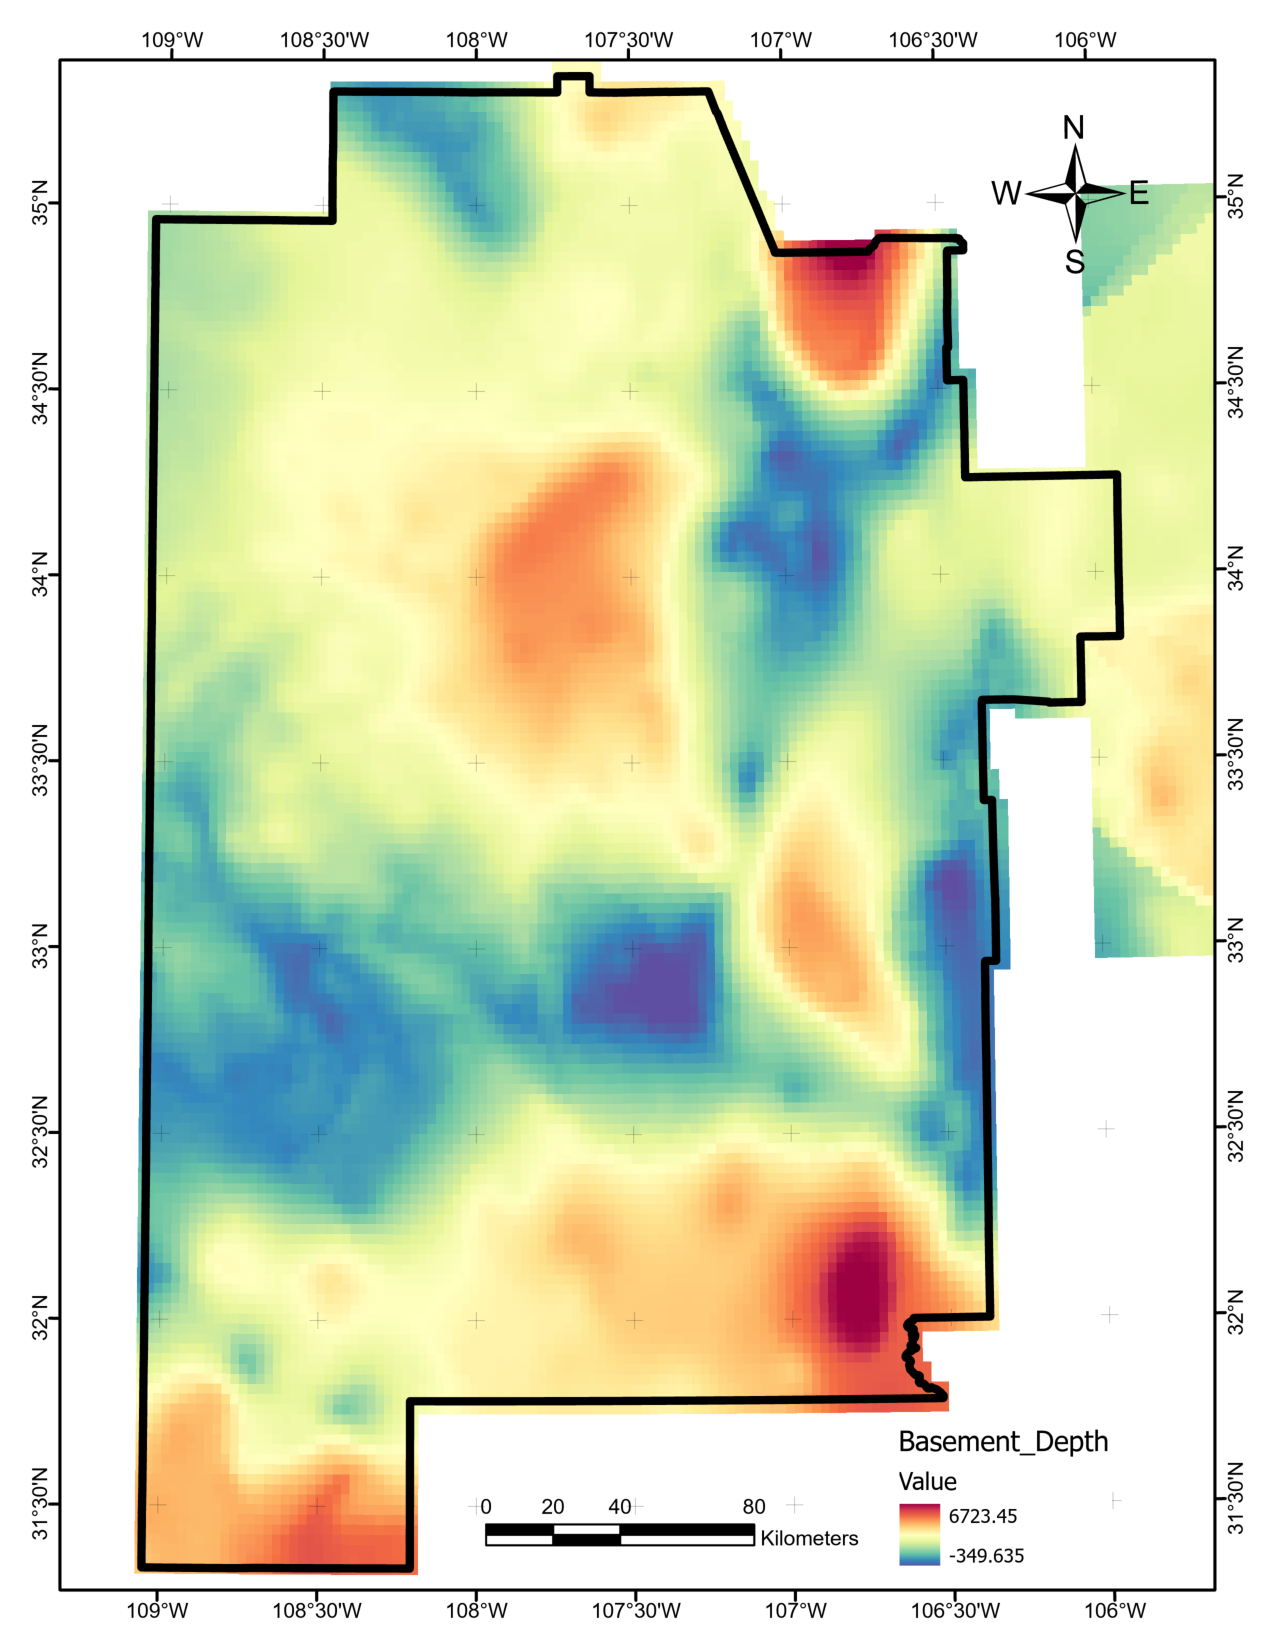
\includegraphics[width=0.75\linewidth]{templates/images/Figure-BasementDepth.pdf}
\caption[Basement depth data layer]{Basement depth data layer. Units are in meters. Layer is based on basement elevation raster from \protect\citet{bielicki_hydrogeolgic_2015}.}
\label{fig:feat_basementdepth}
\end{figure}
\pagebreak

\section{Boron Concentration}\label{app:dl_boron}
Measurements of boron concentration were originally assembled by \citet{bielicki_hydrogeolgic_2015} from USGS records, student dissertations, and other sources. These data were downloaded from the NM PFA OpenEI submission \citep{kelley_geothermal_2015} and merged together using ArcGIS and Python to create a single dataframe of 5,686 measurements within the broader Regional Polygon bounds. Restricting data input to the tighter AOI bounds led to artifacts in the interpolation process. Inconsistent spatial distribution of the data, and sometimes significant variation among overlapping values from different measurement years, created a unique challenge for building a GIS layer. An initial attempt to fit and interpolate the data using tuned Gaussian Process models created feature layers with too much local structure and little character away from the input data points. The ArcGIS \textit{Empirical Bayes Kriging} (EBK) routine was selected instead due to its ability to manage coincident data and its high accuracy with smaller data sets compared to ordinary kriging methods. For the final layer, EBK was applied with the empirical data transformation type, a maximum of 100 points in each local model, 100 simulated semivariograms with k-Bessel model type, a standard circular search neighborhood with a radius of 1.1957 (auto-determined), minimum of 10 neighbors, and maximum of 15 neighbors. The output grid cell size was set to 0.01 degrees. Of important note: the calculation option to include all coincident data were selected, so overlapping measurements were considered in generating the final layer (Figure \ref{fig:feat_boron}).
\vfill
\pagebreak

\begin{figure}[H]
\centering
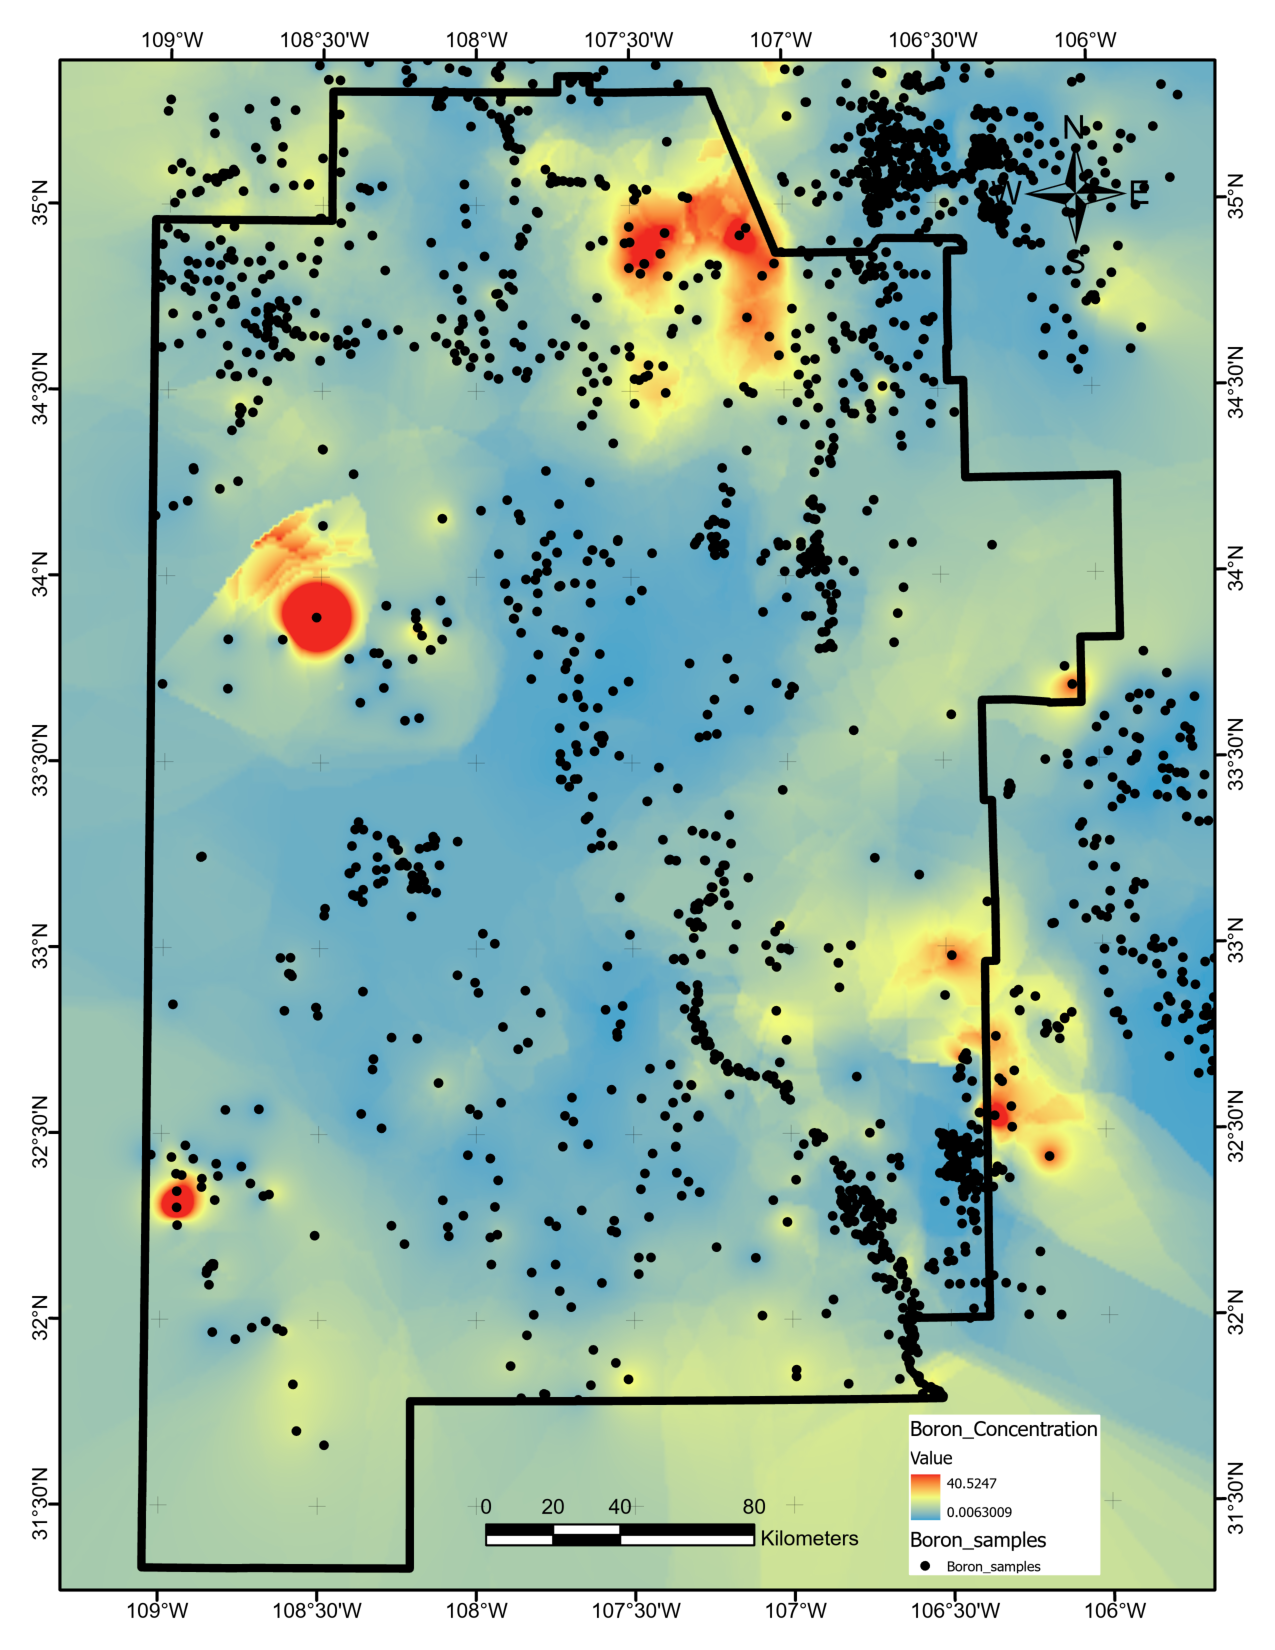
\includegraphics[width=0.75\linewidth]{templates/images/Figure-Boron.pdf}
\caption[Boron concentration data layer]{Boron concentration data layer. Units are in ppm or mg/L. Black dots indicate sample locations in the complete data set compiled by \protect\citet{bielicki_hydrogeolgic_2015}.}
\label{fig:feat_boron}
\end{figure}
\pagebreak

\section{Crustal Thickness}\label{app:dl_crustal_thickness}
In the absence of a more recent seismic study constraining variations in crustal thickness across the study area, the regional map published by \citet{keller_comparative_1991} was used to construct the crustal thickness feature layer. Similar to the procedure described in \citep{pepin_new_2019}, the Keller map was georeferenced in ArcGIS, and thickness contours were manually digitized as polylines. These polylines continued slightly beyond the AOI boundary to ensure proper constraints for surface creation without artifacts near the AOI edges. The ArcGIS function \textit{Feature to 3D by Attribute} converted the polylines into 3-D contours, and \textit{Topo to Raster} interpolated the contours into a continuous final grid. Since the Keller map was derived from low-resolution seismic lines from the 1960s-1980s, the result is a very low frequency approximation for crustal thickness variations associated with the Colorado Plateau and Rio Grande Rift provinces. As such, a slightly larger cell size of 0.025 degrees was used than for other layers. Additional parameter choices included: margin in the cells of 20, smallest z value for interpolation of 25, largest z value for the interpolation of 55, drainage enforcement, and maximum iterations of 20. The final layer is shown in Figure \ref{fig:feat_crust}.
\vfill
\pagebreak

\begin{figure}[H]
\centering
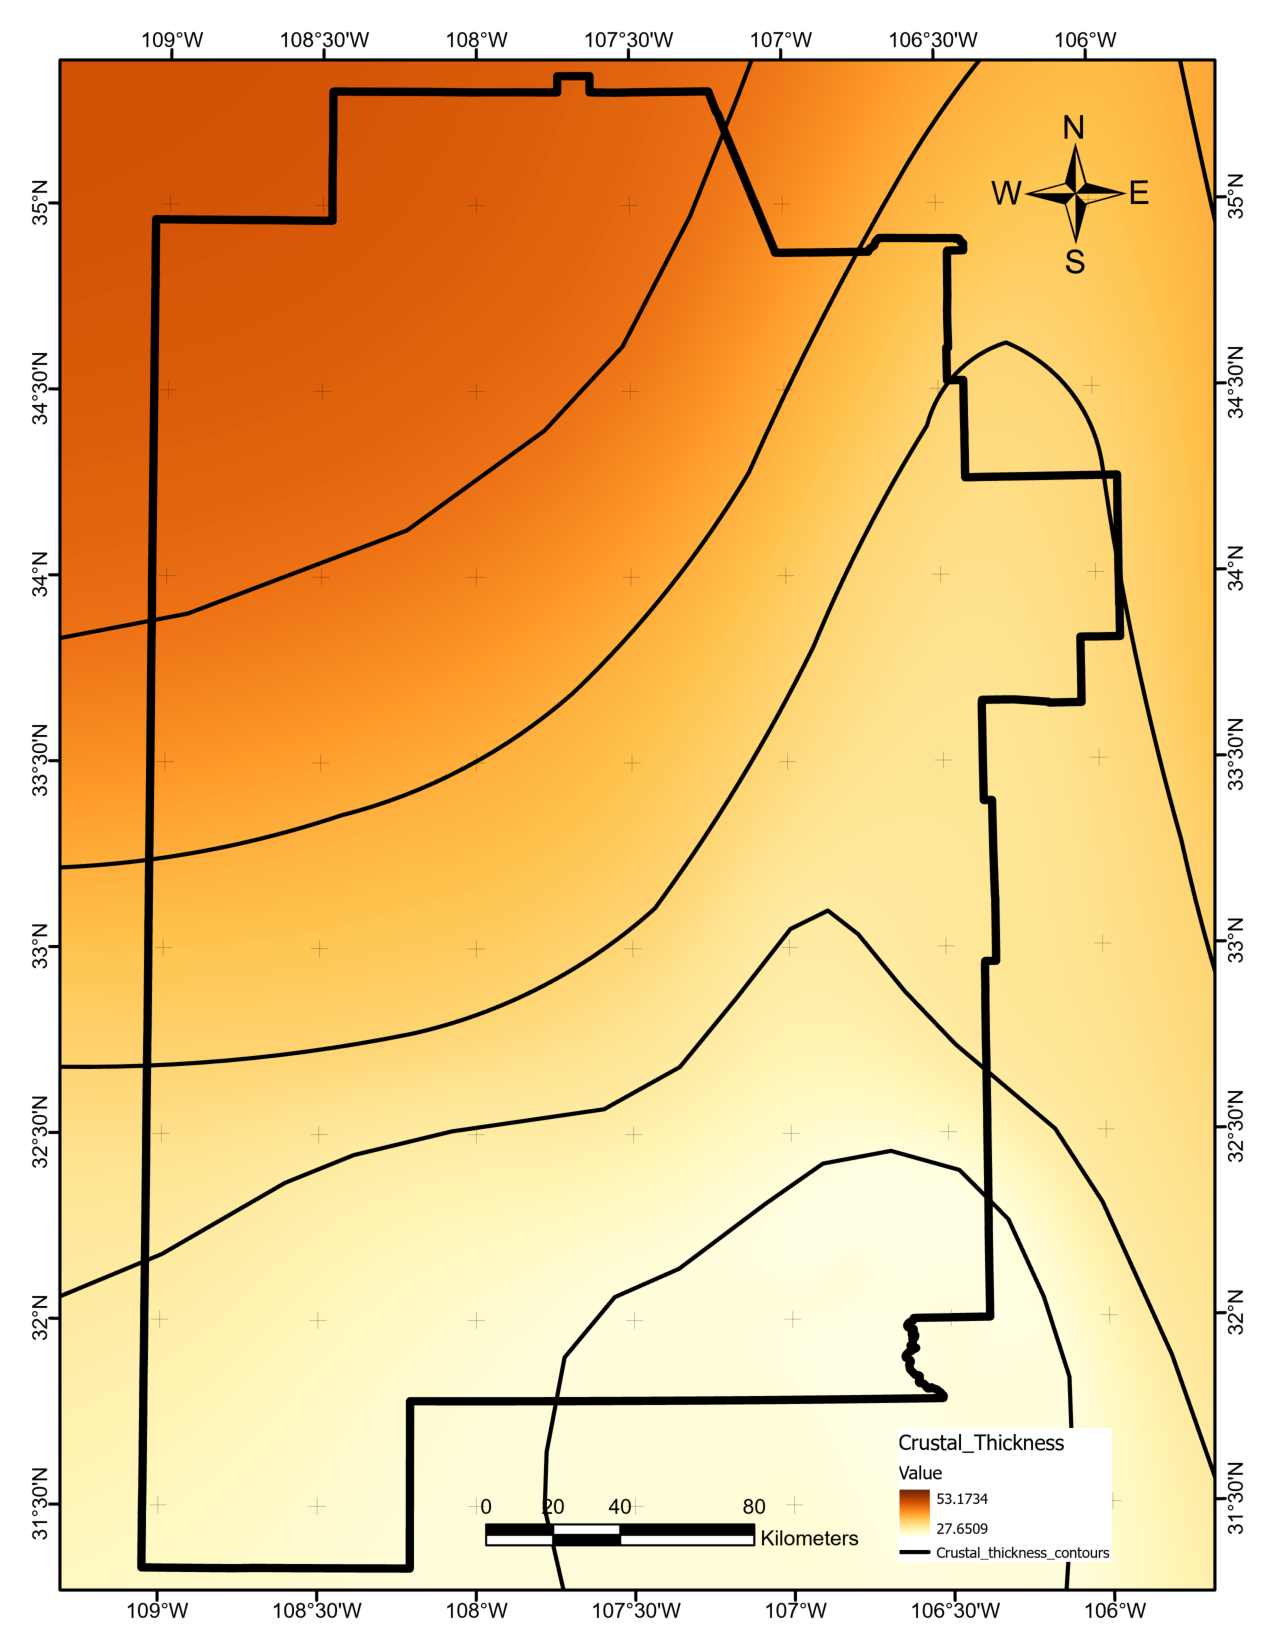
\includegraphics[width=0.75\linewidth]{templates/images/Figure-CrustalThickness.pdf}
\caption[Crustal thickness data layer]{Crustal thickness data layer. Units are in kilometers. Black lines trace the contours digitized from \protect\citet[Figure 4,][]{keller_comparative_1991}.}
\label{fig:feat_crust}
\end{figure}
\pagebreak

\section{Drainage Density}\label{app:dl_drainage_density}
Drainage polyline data comes from the \citet{bielicki_hydrogeolgic_2015} PFA OpenEI submission \citep{kelley_geothermal_2015}. The data were downloaded and imported into ArcGIS, then compared to the DEM layer for quality control. A couple of methods were attempted in order to transform this feature into a continuous-valued layer with full map coverage. First, the polylines were converted to points with 500 m sampling. This point set was loaded into a Python script, which used a grid search routine to determine the best radius for a Gaussian KDE routine available in the scikit-learn package \citep{pedregosa_scikit-learn_2011}. Ten-fold cross validation was employed, which splits the data into 10 subsets and interchangeably trains on 9, tests on one to get an average performance score. Based on a calculation of the negative log likelihood, the best radius was found to be 45,600 m. However, when the kernel density operation is applied to the data with this radius, the map shows a central blob of high density, which falls off toward the sides of the survey. With such a large kernel radius, edge effects come into play since no drainage polylines were available outside of the AOI boundary. Furthermore, the conversion of line data to points for this method disregards the spatial relationships of the connected line data. The ArcGIS \textit{Kernel Density} operation, which handles line data and suggests a kernel radius, produced a layer with more reasonable density relationships by visual inspection. The final drainage density layer used an output cell size of 0.0025 degrees and an auto-determined search radius of 0.272 (Figure \ref{fig:feat_drainage}).
\vfill
\pagebreak

\begin{figure}[H]
\centering
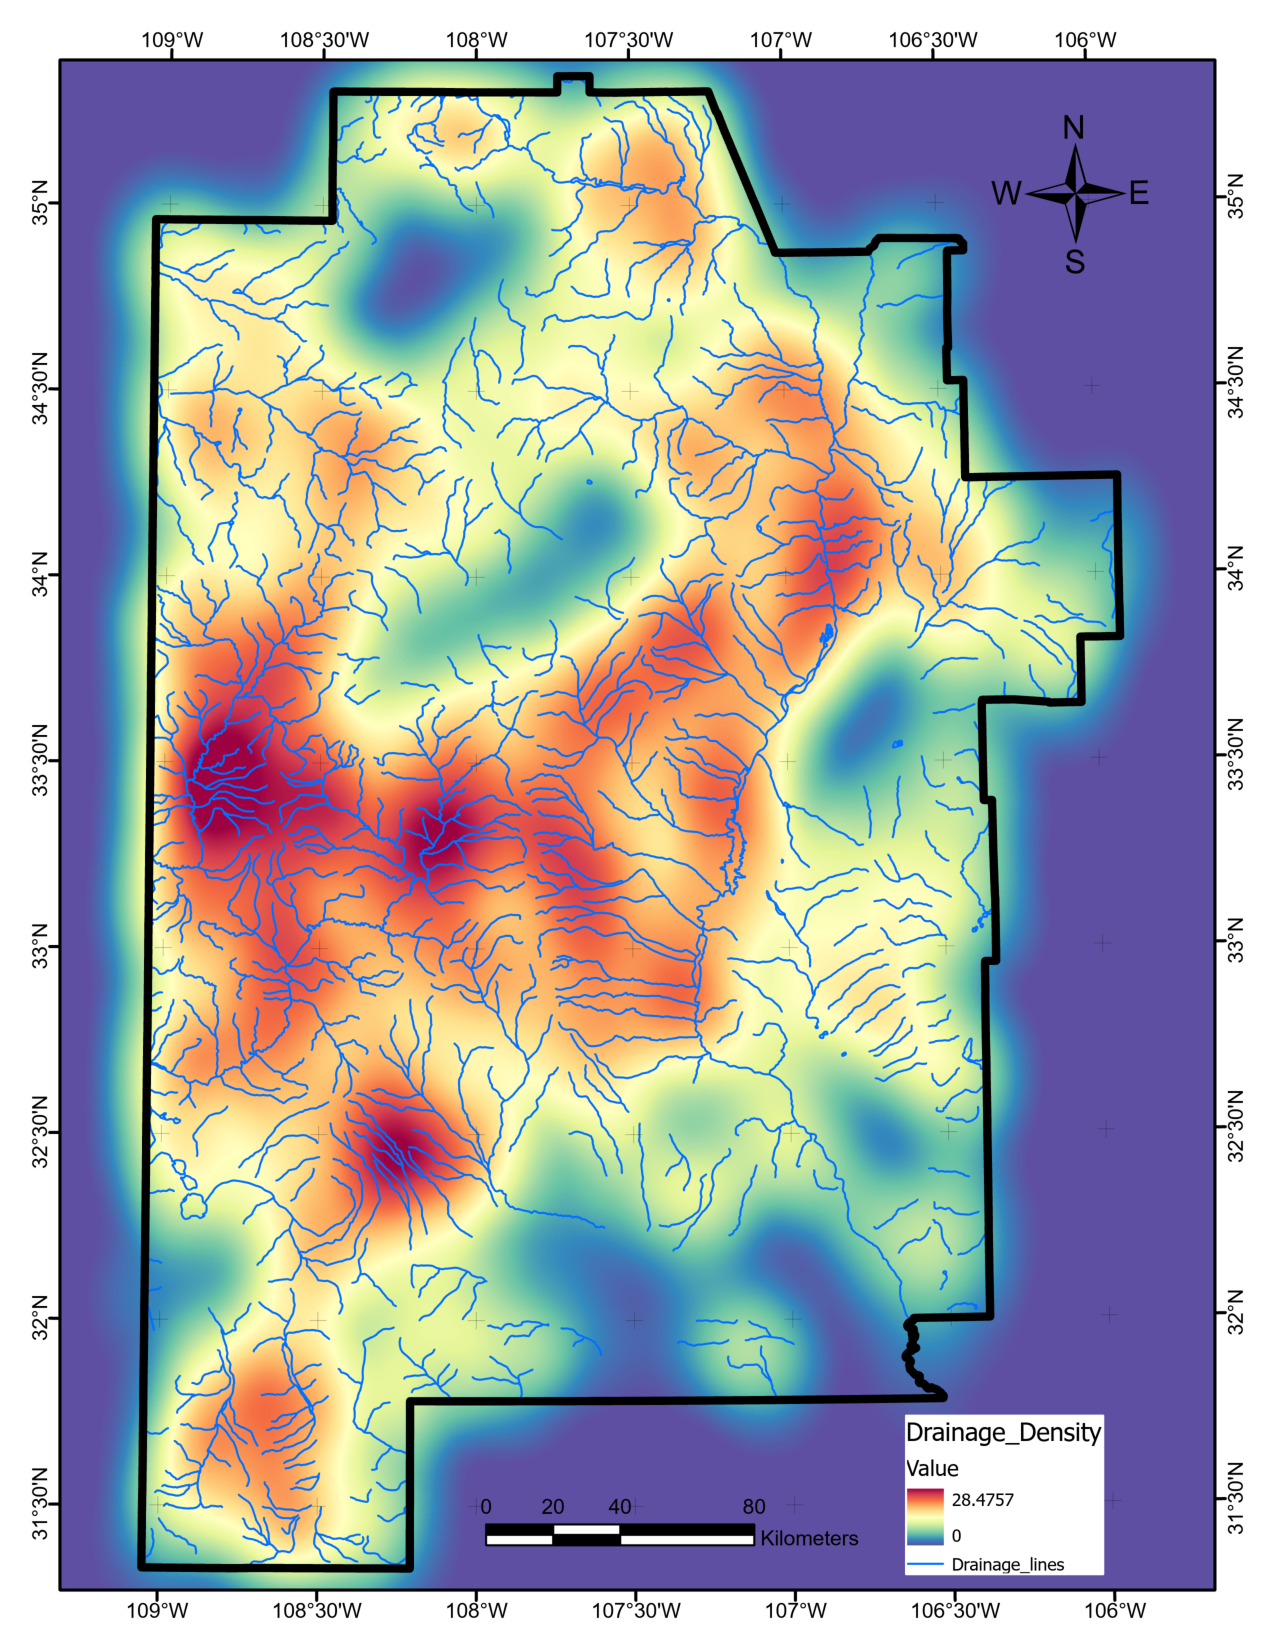
\includegraphics[width=0.75\linewidth]{templates/images/Figure-DrainageDensity.pdf}
\caption[Drainage density data layer]{Drainage density data layer. Units are in degrees/degrees$^2$. Blue lines show the drainage polyline data set from \protect\citet{bielicki_hydrogeolgic_2015}.}
\label{fig:feat_drainage}
\end{figure}
\pagebreak

\section{Earthquake Density}\label{app:dl_eq_density}
\begin{wrapfigure}{R}{0.5\linewidth}
\centering
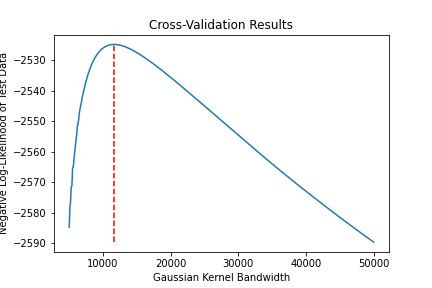
\includegraphics[scale=0.6]{templates/images/Figure-Earthquakes_kde_gridsearchcv_result.png}
\singlespacing
\caption[Earthquake density parameter tuning]{Cross-validation results for earthquake KDE. Red dashed line indicates maximum negative log likelihood value identifying the best kernel radius.}
\label{fig:EQ_cv}
\end{wrapfigure}
Following the procedure outlined by \citet{pepin_new_2019}, an earthquake data set for Southwestern New Mexico was created by combining historical earthquake catalogs for 1869-1998 \citep{sanford_earthquake_2002}, 1999-2004 \citep{sanford_earthquake_2006}, and 2005-2009 \citep{pursley_earthquake_2013} with data pulled from the USGS Earthquake catalog \citep{usgs_earthquake_2021} through to January 2021. All events were combined into a single dataframe in Python, and event duplicates were removed. The final catalog, cropped to the Regional Polygon boundary, consists of 2,539 events spanning 1962-2020. This point set was loaded into a KDE Python script, which used a grid search to determine the best radius for the scikit-learn \textit{KernelDensity} routine \citep{pedregosa_scikit-learn_2011}. Ten-fold cross validation was employed, which splits the data into 10 subsets and then interchangeably trains on 9 and tests on one to get an average performance score. The maximum negative log likelihood indicates a best radius value of 11,600 m (Figure \ref{fig:EQ_cv}). 

KDE values calculated at each AOI mesh grid point location were loaded into ArcGIS, and the \textit{Kriging} function created a final surface for plotting purposes. \textit{Kriging} parameters included: spherical semivariogram model, lag size of 1e-6, variable search radius with 12-point requirement, and output cell size of 0.01. The final layer is shown in Figure \ref{fig:feat_EQ_density}.
\vfill
\pagebreak

\begin{figure}[H]
\centering
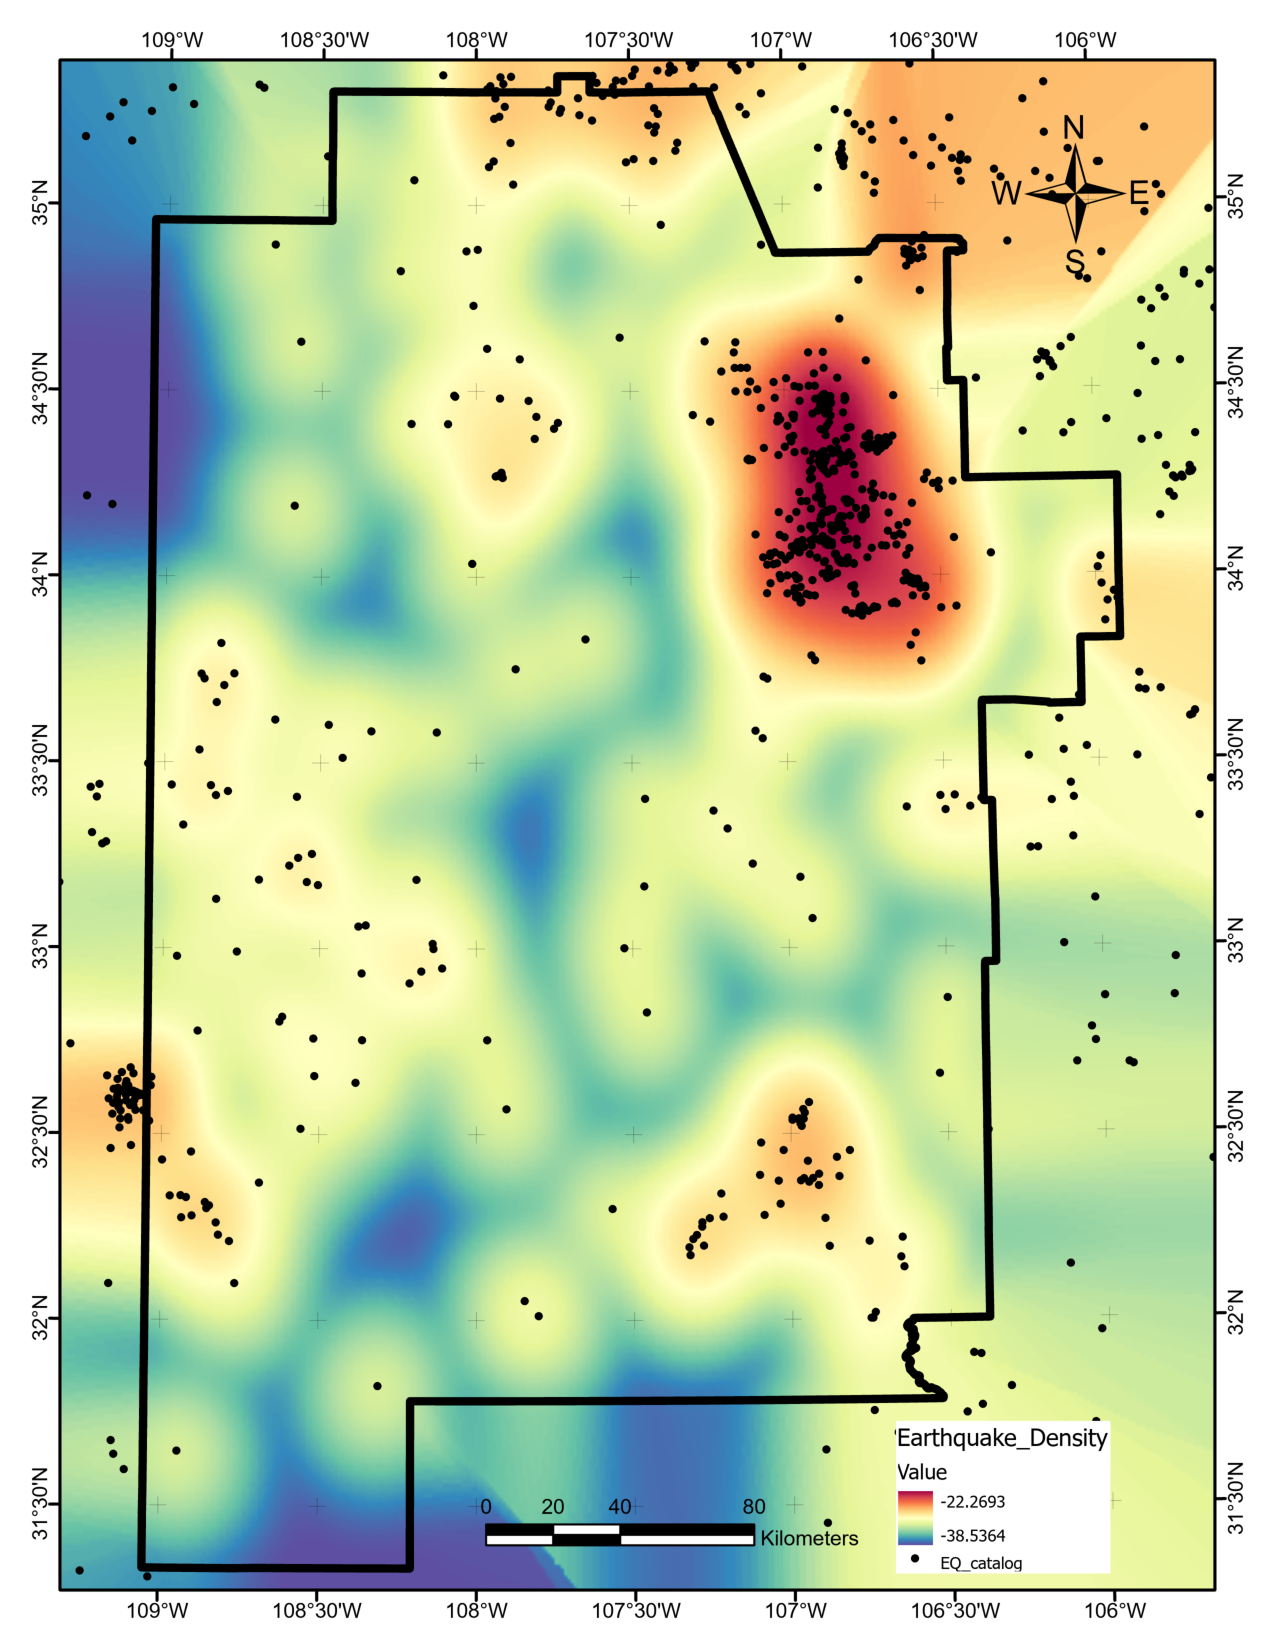
\includegraphics[width=0.75\linewidth]{templates/images/Figure-EarthquakeDensity.pdf}
\caption[Earthquake density data layer]{Earthquake density data layer. Units are in log(points/km$^2$). Black dots indicate earthquake locations.}
\label{fig:feat_EQ_density}
\end{figure}
\pagebreak

\section{Gamma Ray Dose Rate}\label{app:dl_gamma_dose}
Aerial gamma ray surveys conducted across the United States in the late 1970-1980s allowed for the construction of Potassium concentration (K, in percent K), Uranium concentration (eU, in ppm), and Thorium concentration (eTh in ppm) maps, which tie back to mineralogy and hence are a proxy for stratigraphy. These measures collectively define the absorbed dose rate, which can be calculated from the following equation: $D = 13.2 K + 5.48 eU + 2.72 eTh$ \citep{duval_terrestrial_2005}.

The absorbed dose rate for West Central USA was downloaded from the USGS Open-File Report 2005-1413 website \citep{duval_terrestrial_2005}, loaded into ArcGIS, and cropped to the Regional Polygon bounds. A data gap in the vicinity of the White Sands Missile Range to the southeast of the study area necessitated layer interpolation using kriging. Grid values were extracted using the AOI mesh grid, then passed through the ArcGIS \textit{Kriging} function to create the final layer based on the following preferred parameters: spherical semivariogram model, auto-determined lag size of 0.097, and a variable search radius with a 4-point requirement (Figure \ref{fig:feat_gamma}).
\vfill
\pagebreak

\begin{figure}[H]
\centering
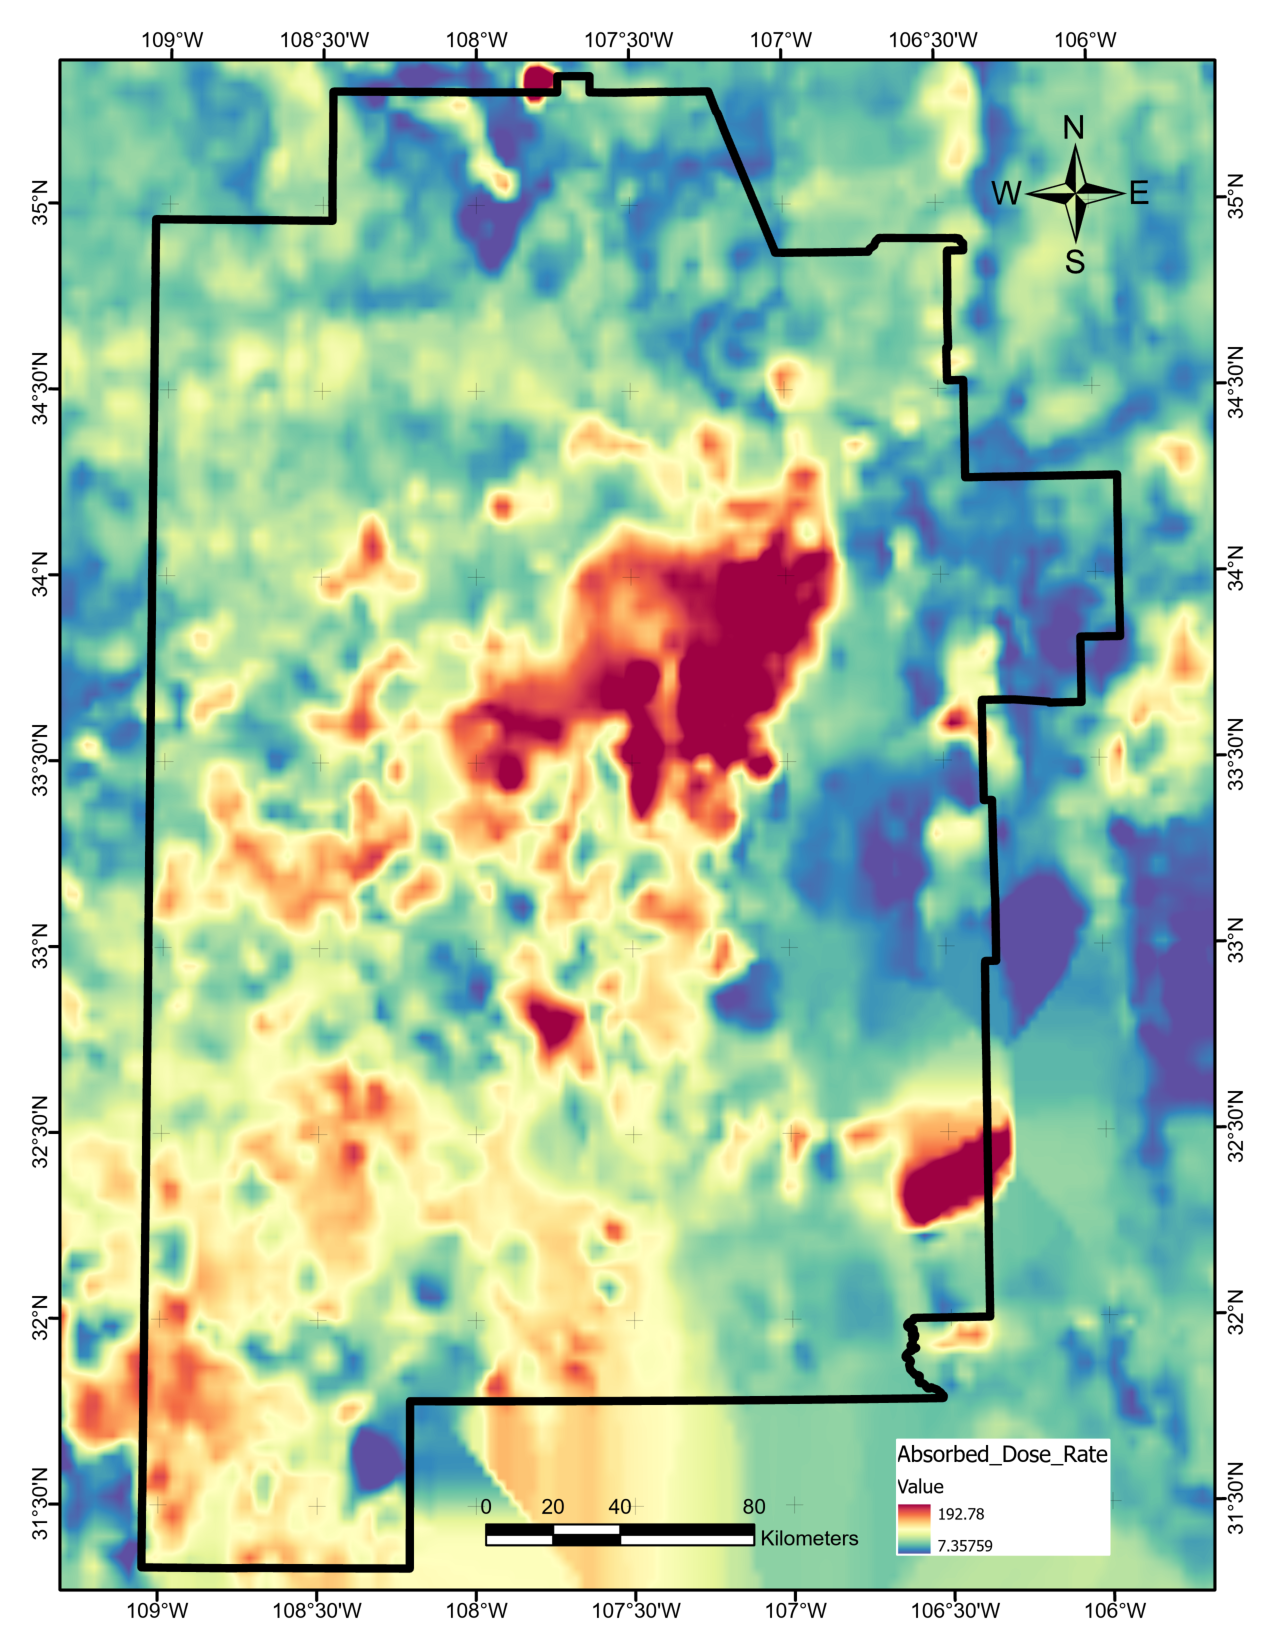
\includegraphics[width=0.75\linewidth]{templates/images/Figure-AbsorbedDose.pdf}
\caption[Absorbed dose rate data layer]{Absorbed dose rate data layer. Units are in nanoGrays/hour (nGy/hr). Original data from USGS Open-File Report 2005-1413 \protect\citep{duval_terrestrial_2005}.}
\label{fig:feat_gamma}
\end{figure}
\pagebreak

\section{Geodetic Strain Rate}\label{app:dl_strain_rate}
GPS stations worldwide record local movements in the crust. These movements can highlight inflation or subsidence of the surface, fault motions, or plate tectonic activity. The spatial derivative of crustal velocities is termed the strain rate, which gives an indication of the accumulation of strain in an area. More concretely, it defines the speed with which the crust is deforming, and can be treated as a proxy for earthquake potential since slip occurs due to the accumulation of strain \citep{gem_strain_2014}. The Global Strain Rate Model (GSRM) v.2.1 provides a model for strain rate based on over 22,000 measurements from over 18,000 locations around the world \citep{kreemer_geodetic_2014}. The output of this model was downloaded from the University of Nevada Reno Geodetic Laboratory host site \citep{kreemer_global_2020}. GSRM describes elements of the full strain tensor at a $0.1^\circ$ resolution. The magnitude or second invariant of the strain tensor can combine these elements into a single value \citep{kreemer_geodetic_2014}:

\begin{equation}\label{eq:strainratemagnitude}
\left\lVert\dot{\epsilon}\right\rVert = \sqrt{\dot{\varepsilon}_{\phi\phi}^2+\dot{\varepsilon}_{\theta\theta}^2+2\dot{\varepsilon}_{\phi\theta}^2}
\end{equation}

Due to the size of the GSRM model file and complexity of this calculation, the data were first loaded into Python, cropped to the Regional Polygon bounds, and the strain rate magnitude was calculated for each point. These data were then loaded into ArcGIS and gridded using the \textit{Spline} function for a smooth interpolation of the coarser GSRM grid. The final layer  was created using the following \textit{Spline} parameters: regularized type, weight of 0.1, 4-point requirement, and cell size of 0.025 degrees (Figure \ref{fig:feat_strain}).
\vfill
\pagebreak

\begin{figure}[H]
\centering
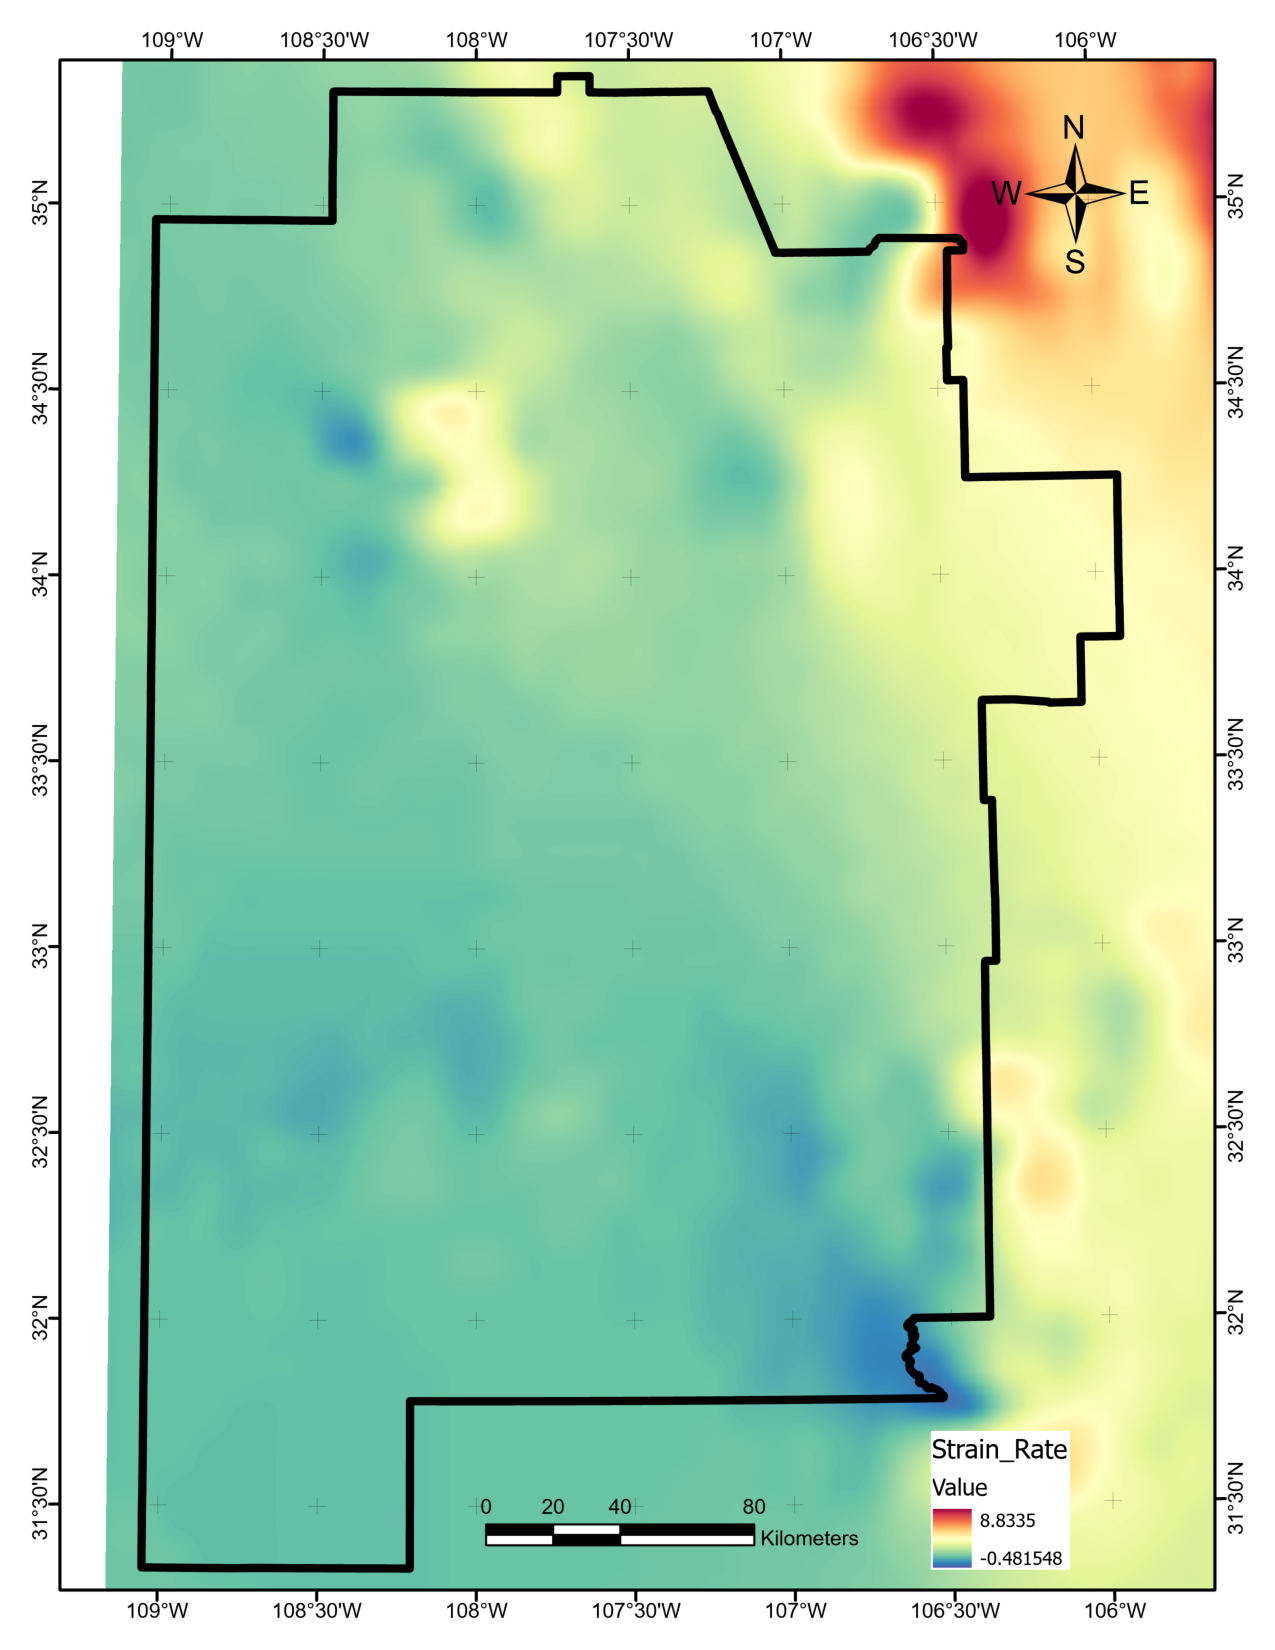
\includegraphics[width=0.75\linewidth]{templates/images/Figure-StrainRate.pdf}
\caption[Geodetic strain rate data layer]{Geodetic strain rate data layer. Units are in $10^-9$\ m/(m$\cdot$yr). Layer is based on data from \protect\citet{kreemer_geodetic_2014}.}
\label{fig:feat_strain}
\end{figure}
\pagebreak

\section{Gravity Anomaly}\label{app:dl_grav_anomaly}
Terrain-corrected gravity anomaly data available from the University of Texas El Paso \citep{utep_gravity_2011} were used in both the PFA analysis \citep{bielicki_hydrogeolgic_2015} and cluster analysis \citep{pepin_new_2019} for Southwestern NM. The data layer from \citet{bielicki_hydrogeolgic_2015} was downloaded from their OpenEI submission \citep{kelley_geothermal_2015} and loaded into ArcGIS. This layer required no further processing (Figure \ref{fig:feat_gravity}).

\begin{figure}[H]
\centering
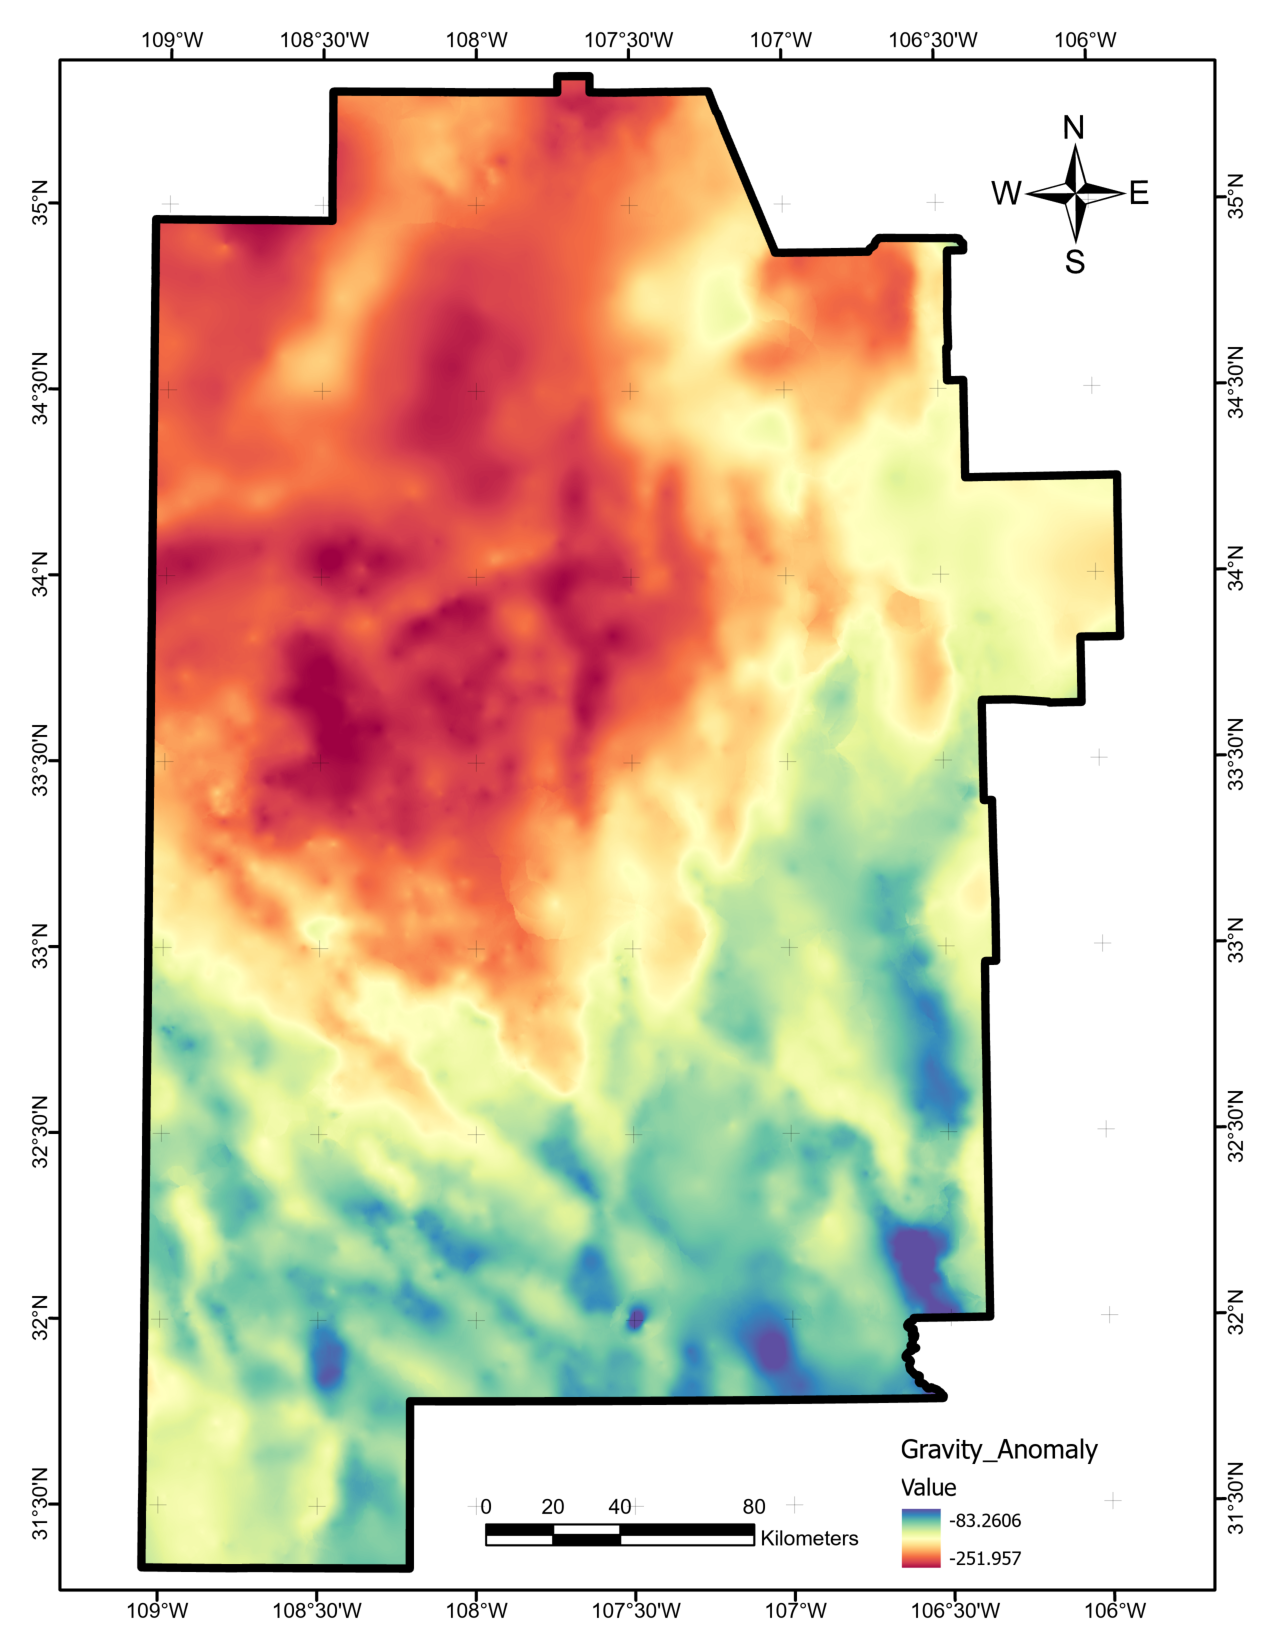
\includegraphics[width=0.75\linewidth]{templates/images/Figure-GravityAnomaly.pdf}
\caption[Gravity anomaly data layer]{Gravity anomaly data layer. Units are in milligals (mGal). Raster originally created by \protect\citet{bielicki_hydrogeolgic_2015}.}
\label{fig:feat_gravity}
\end{figure}
\pagebreak

\section{Gravity Anomaly Gradient}\label{app:dl_grav_gradient}
Gravity anomaly gradient was calculated using the ArcGIS \textit{Slope} function on the final Gravity Anomaly raster. Parameters used to create the final layer include: geodesic method, z unit of meters, and output measurement of degrees (Figure \ref{fig:feat_gravity_gradient}).

\begin{figure}[H]
\centering
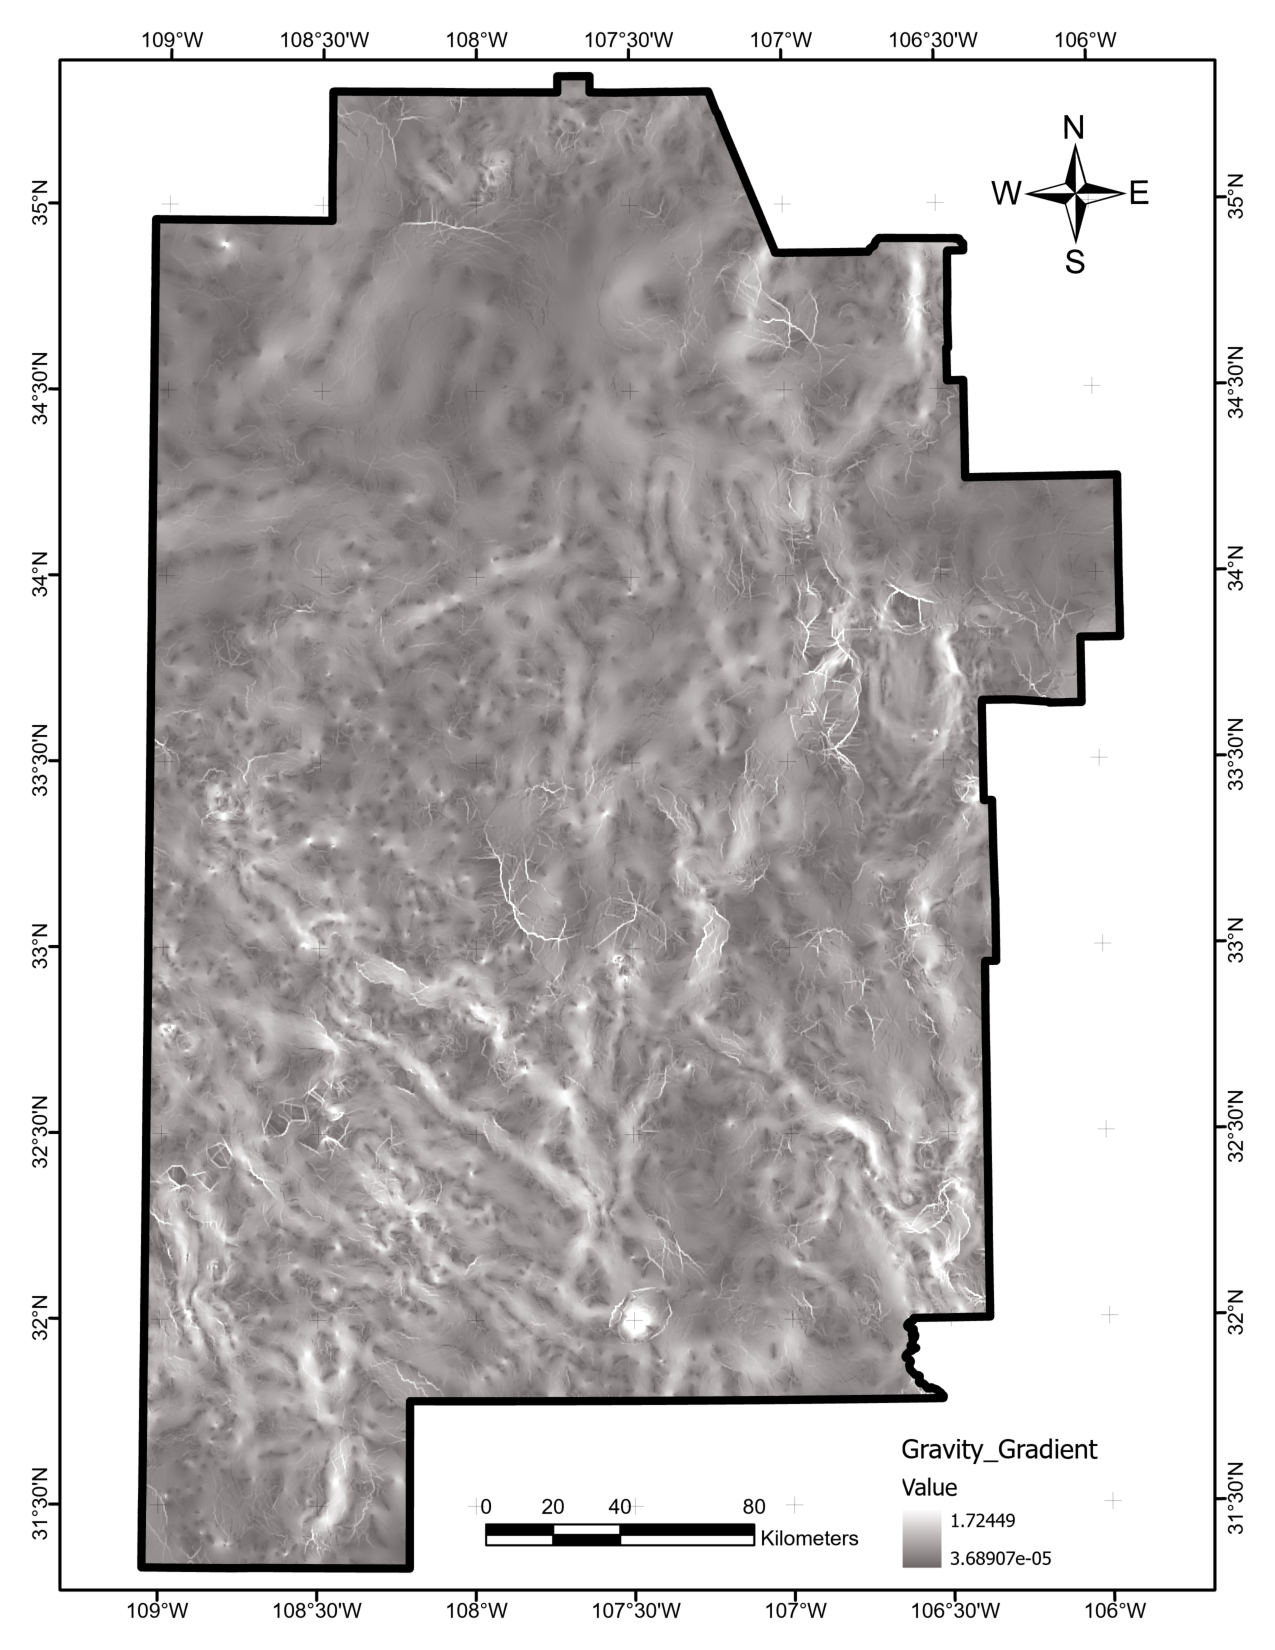
\includegraphics[width=0.75\linewidth]{templates/images/Figure-GravityGradient.pdf}
\caption[Gravity anomaly gradient data layer]{Gravity anomaly gradient data layer. Units are in mGal/degrees.}
\label{fig:feat_gravity_gradient}
\end{figure}
\pagebreak

\section{Heat Flow}\label{app:dl_heat_flow}
The \(0.5^\circ\times0.5^\circ\) resolution heat flow model from \citet{lucazeau_analysis_2019} offers coarse coverage across the Southwestern NM AOI. This model was downloaded directly from the supporting information section of the publication page \citep{lucazeau_analysis_2019}, imported into ArcGIS, and cropped to the Regional Polygon boundaries. After testing several gridding algorithms for a smooth representation of this sparse data, the ArcGIS \textit{Topo to Raster} function produced the best results. The parameters for creating the final layer include: tolerance-1 of 2.5, tolerance-2 of 100, drainage enforcement, contour input data, and output cell size of 0.01 (Figure \ref{fig:feat_heatflow}).
\vfill
\pagebreak

\begin{figure}[H]
\centering
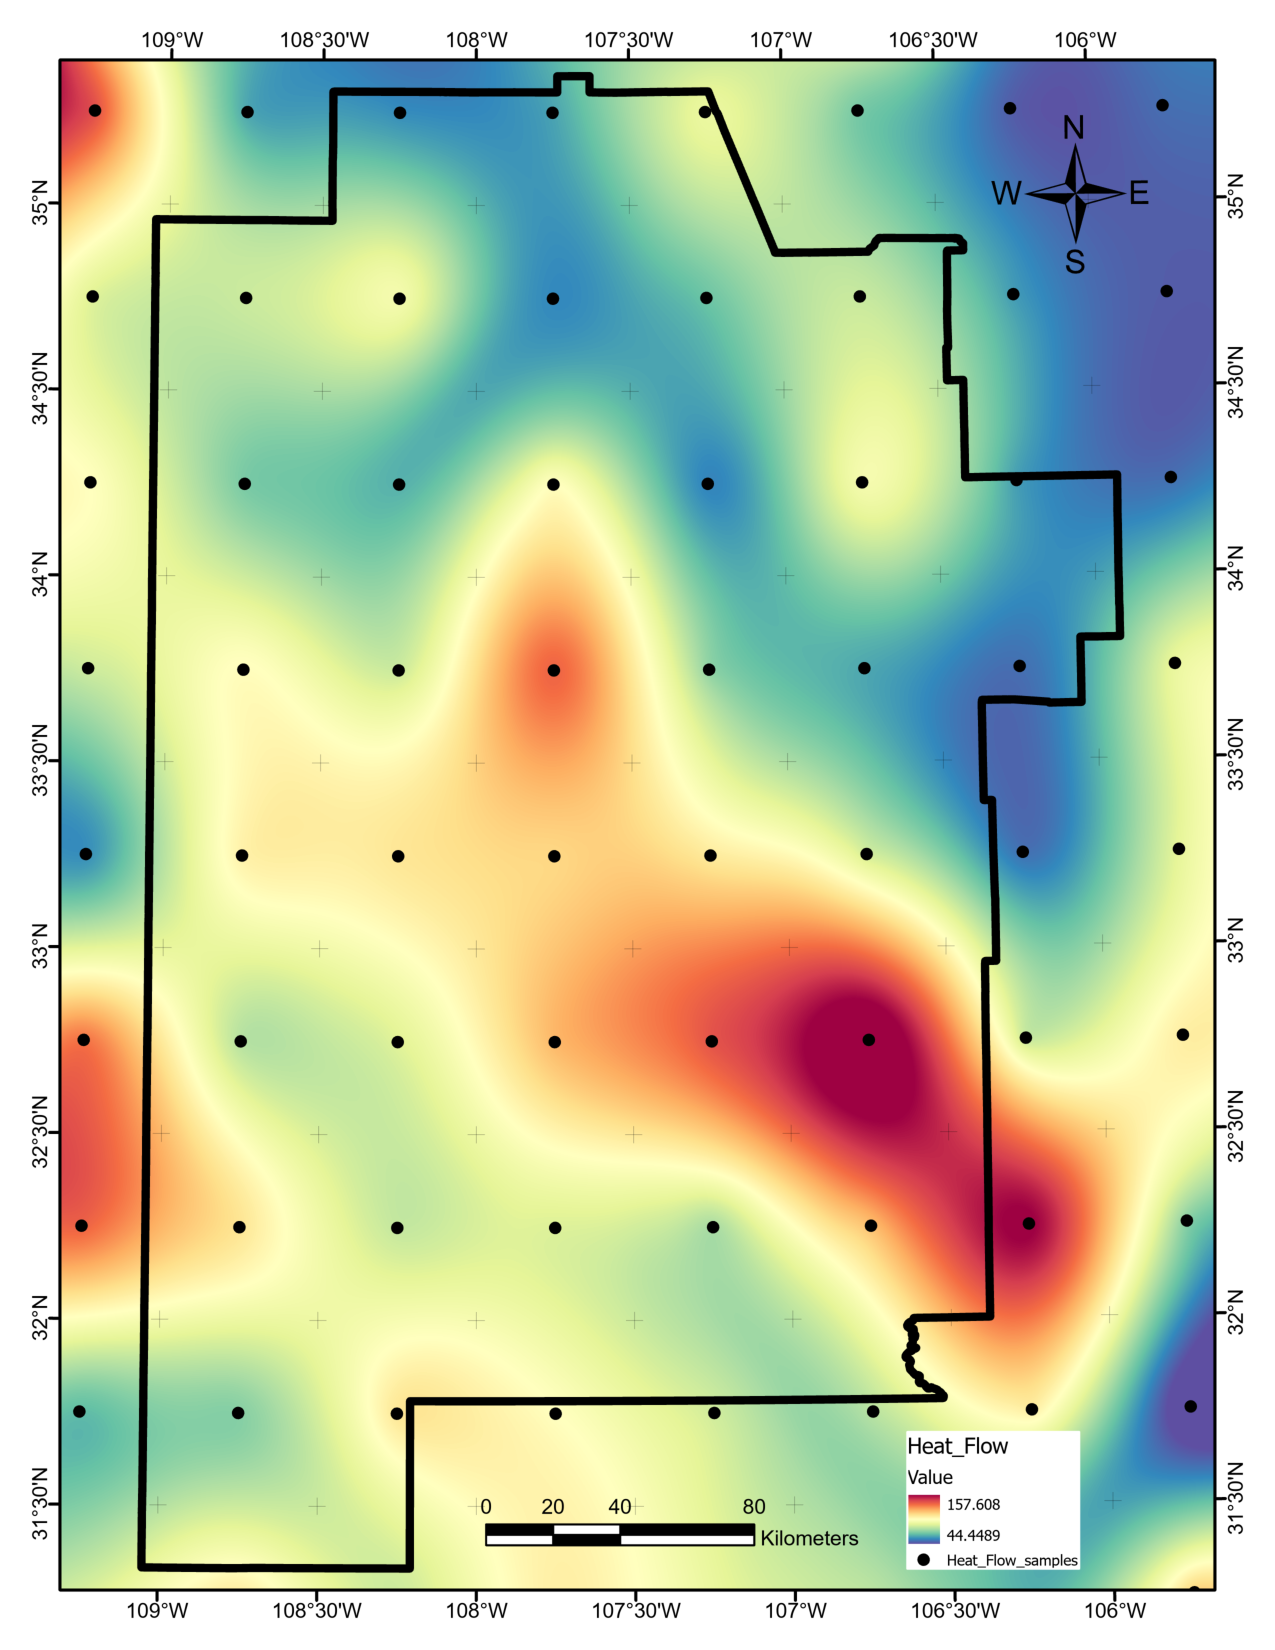
\includegraphics[width=0.75\linewidth]{templates/images/Figure-HeatFlow.pdf}
\caption[Heat flow data layer]{Heat flow data layer. Units are in W/m-K. Black dots mark the original source data points from \protect\citet{lucazeau_analysis_2019}.}
\label{fig:feat_heatflow}
\end{figure}
\pagebreak

\section{Lithium Concentration}\label{app:dl_lithium}
Measurements of lithium concentration were originally assembled by \citet{bielicki_hydrogeolgic_2015} from USGS records, student dissertations, and other sources. These data were downloaded from the NM PFA OpenEI submission \citep{kelley_geothermal_2015} and merged together using ArcGIS and Python to create a single dataframe of 3,595 measurements within the broader Regional Polygon bounds. Restricting data input to the tighter AOI bounds led to artifacts in the interpolation process. As described for the Boron Concentration data layer, attempts to model lithium concentration using Gaussian Processes provided unsatisfactory results. Instead, the final layer was generated using the ArcGIS \textit{Empirical Bayes Kriging} routine. Selected parameters include: empirical data transformation type, a maximum of 100 points in each local model, 100 simulated semivariograms with k-Bessel model type, a standard circular search neighborhood with a radius of 1.196 (auto-determined), minimum of 10 neighbors, and maximum of 15 neighbors. The output grid cell size was set to 0.01 degrees. All coincident data were included in the calculation, so any overlapping measurements were considered in generating the final layer (Figure \ref{fig:feat_lithium}).
\vfill
\pagebreak

\begin{figure}[H]
\centering
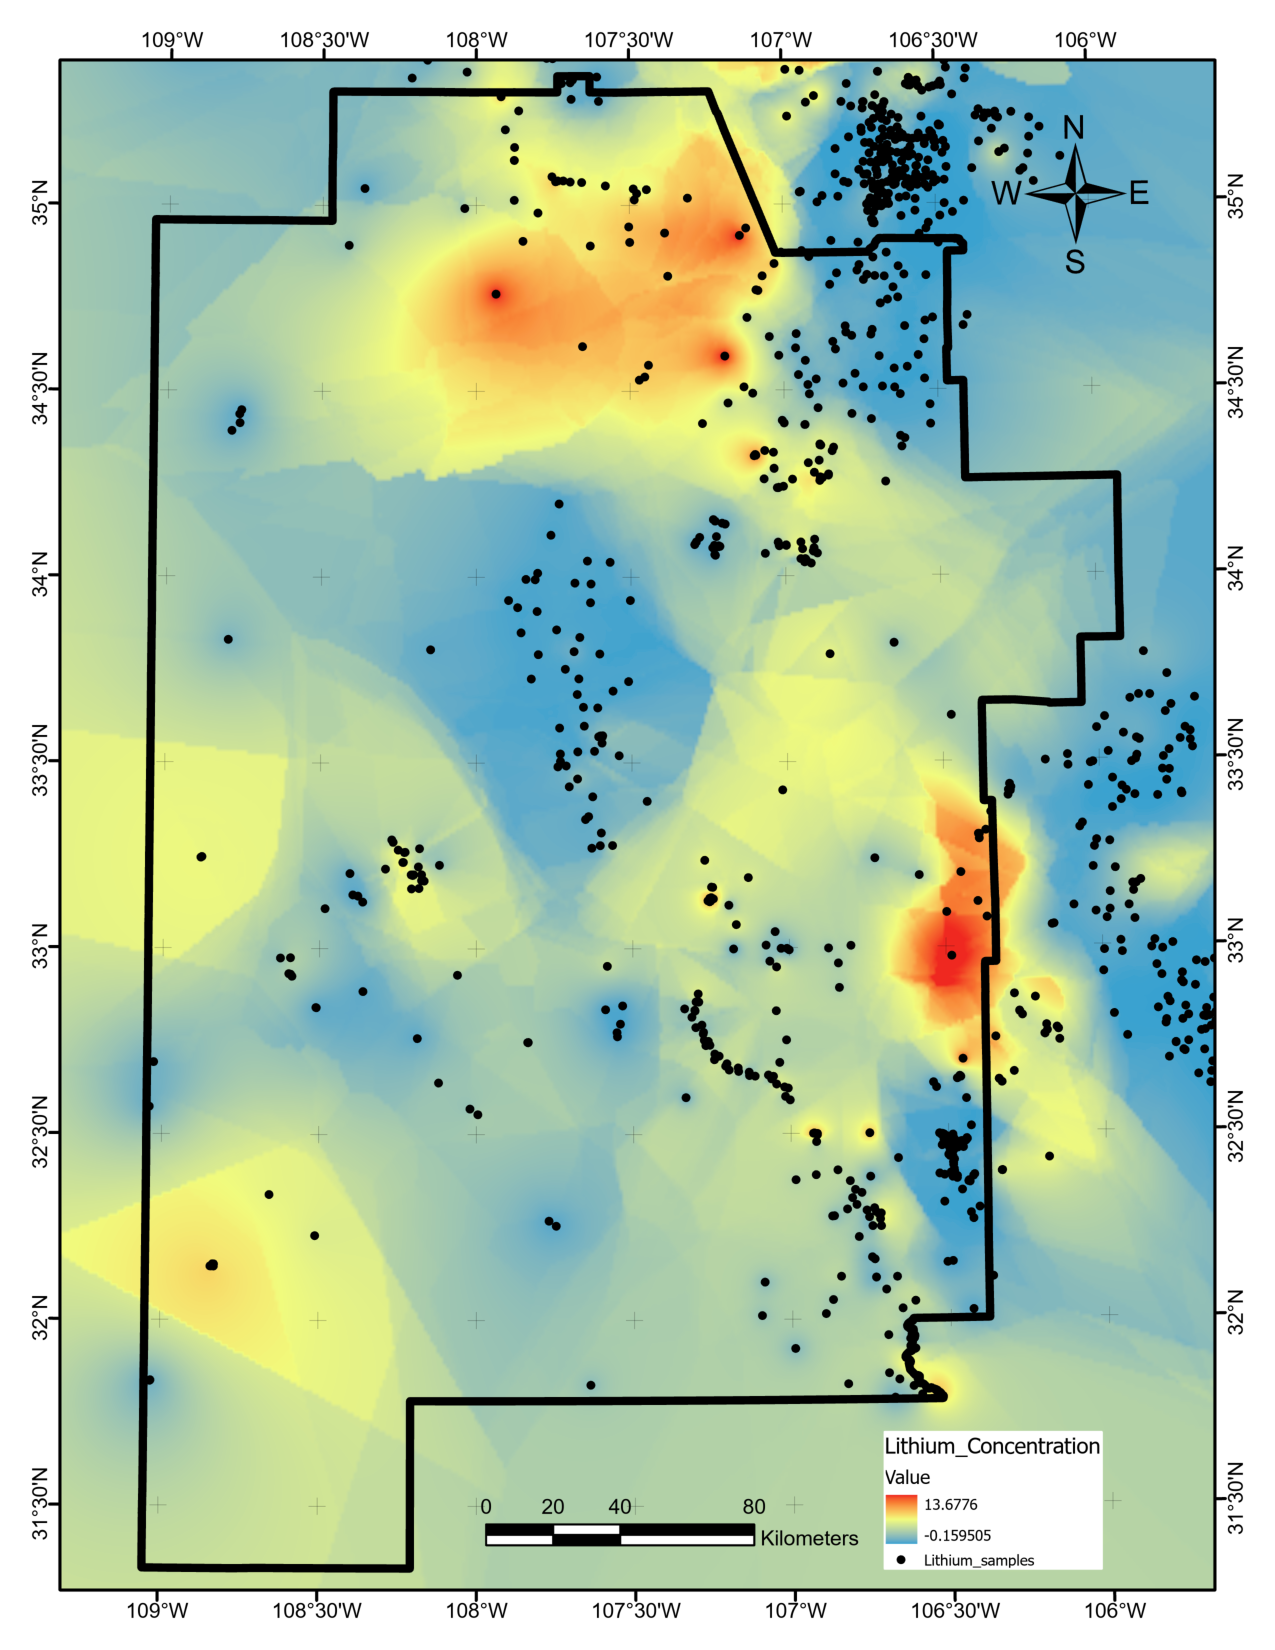
\includegraphics[width=0.75\linewidth]{templates/images/Figure-Lithium.pdf}
\caption[Lithium concentration data layer]{Lithium concentration data layer. Units are in ppm or mg/L. Black dots mark sample locations in the complete data set from \protect\citet{bielicki_hydrogeolgic_2015}}.
\label{fig:feat_lithium}
\end{figure}
\pagebreak

\section{Magnetic Anomaly}\label{app:dl_magnetic_anomaly}
USGS magnetic anomaly data from merged aerial surveys \citep{bankey_digital_2002} were used in both the Southwestern NM PFA analysis \citep{bielicki_hydrogeolgic_2015} and cluster analysis \citep{pepin_new_2019}. After downloading the raster from the PFA OpenEI submission \citep{kelley_geothermal_2015}, it was imported directly into ArcGIS. No further processing was required (Figure \ref{fig:feat_magnetics}).

\begin{figure}[H]
\centering
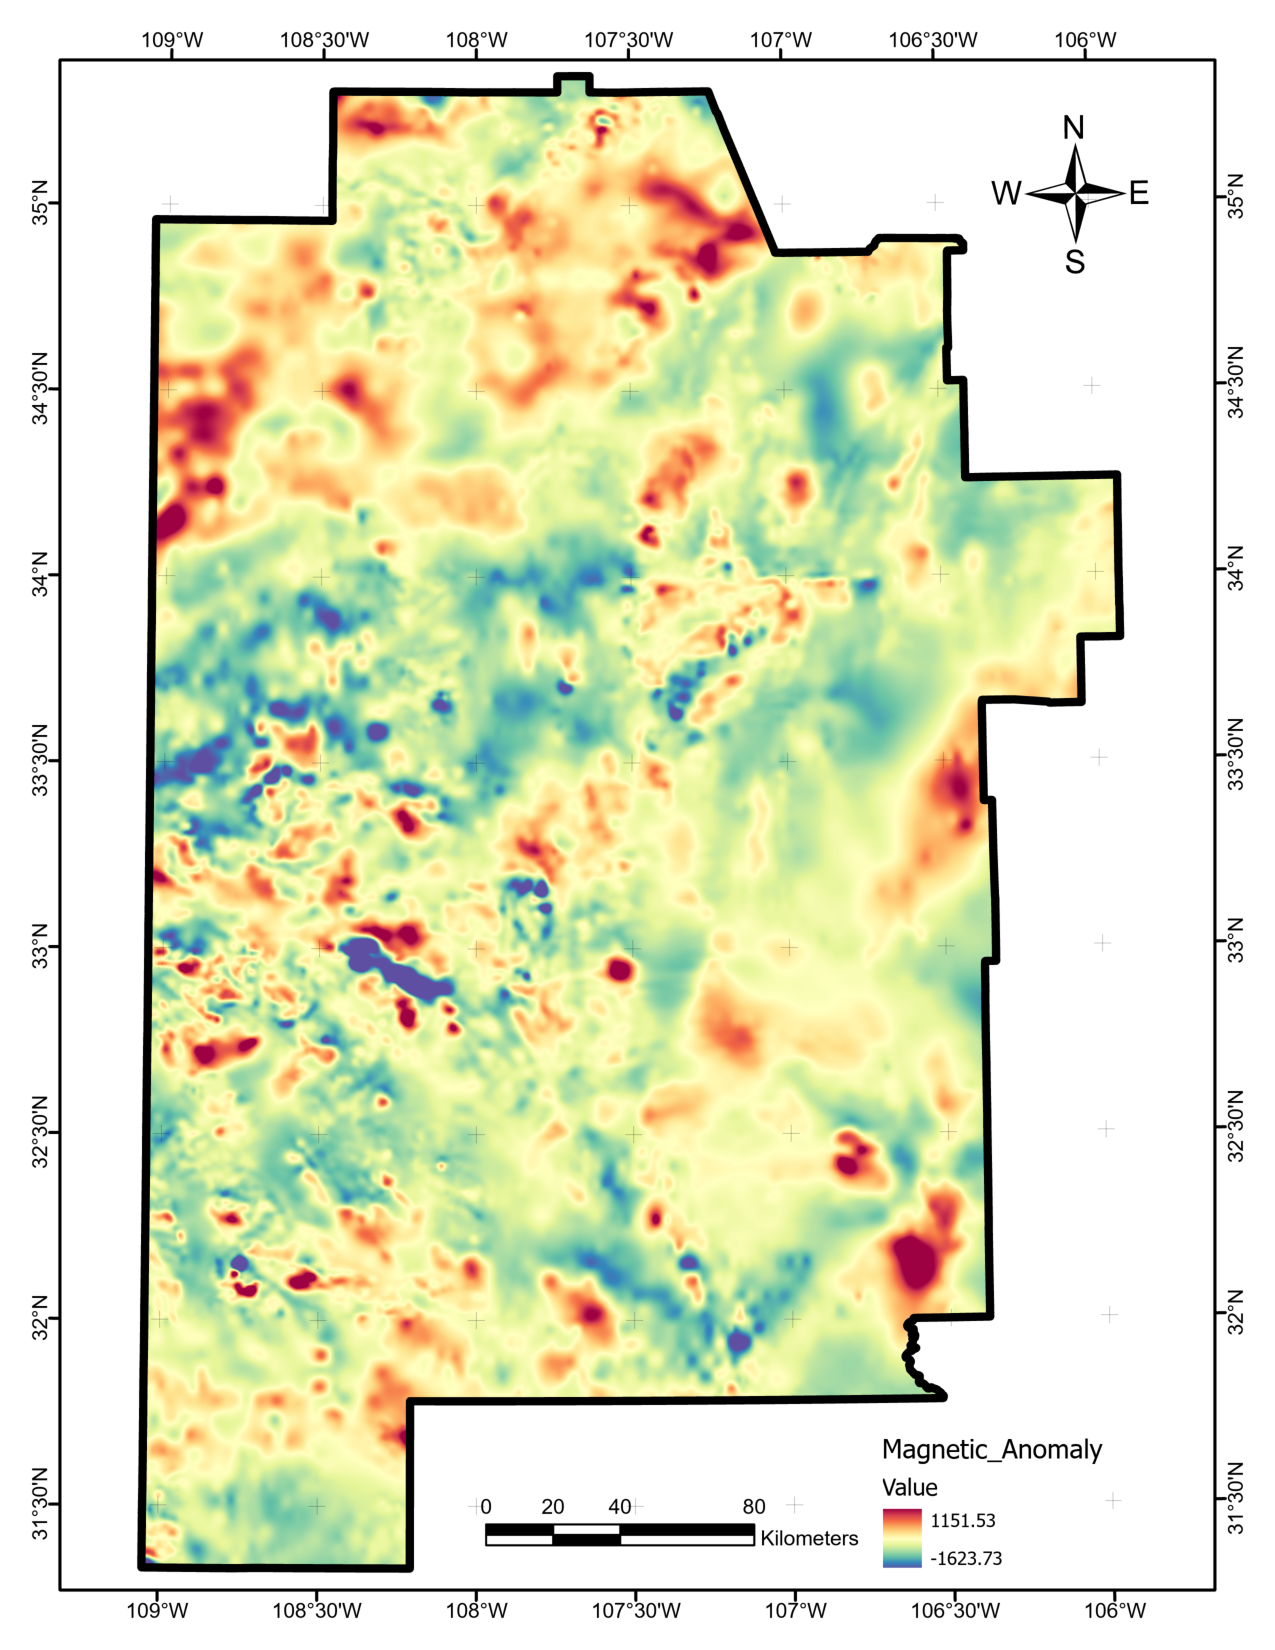
\includegraphics[width=0.75\linewidth]{templates/images/Figure-MagneticAnomaly.pdf}
\caption[Magnetic anomaly data layer]{Magnetic anomaly data layer. Units are in nanoteslas (nT). Raster originally created by \protect\citet{bielicki_hydrogeolgic_2015}.}
\label{fig:feat_magnetics}
\end{figure}
\pagebreak

\section{Magnetic Anomaly Gradient}\label{app:dl_magnetic_gradient}
Magnetic anomaly gradient was calculated using the ArcGIS \textit{Slope} function on the final Magnetic Anomaly raster. Parameters selected to create this layer include: geodesic method, z unit of meters, and output measurement of degrees (Figure \ref{fig:feat_magnetic_gradient}).

\begin{figure}[H]
\centering
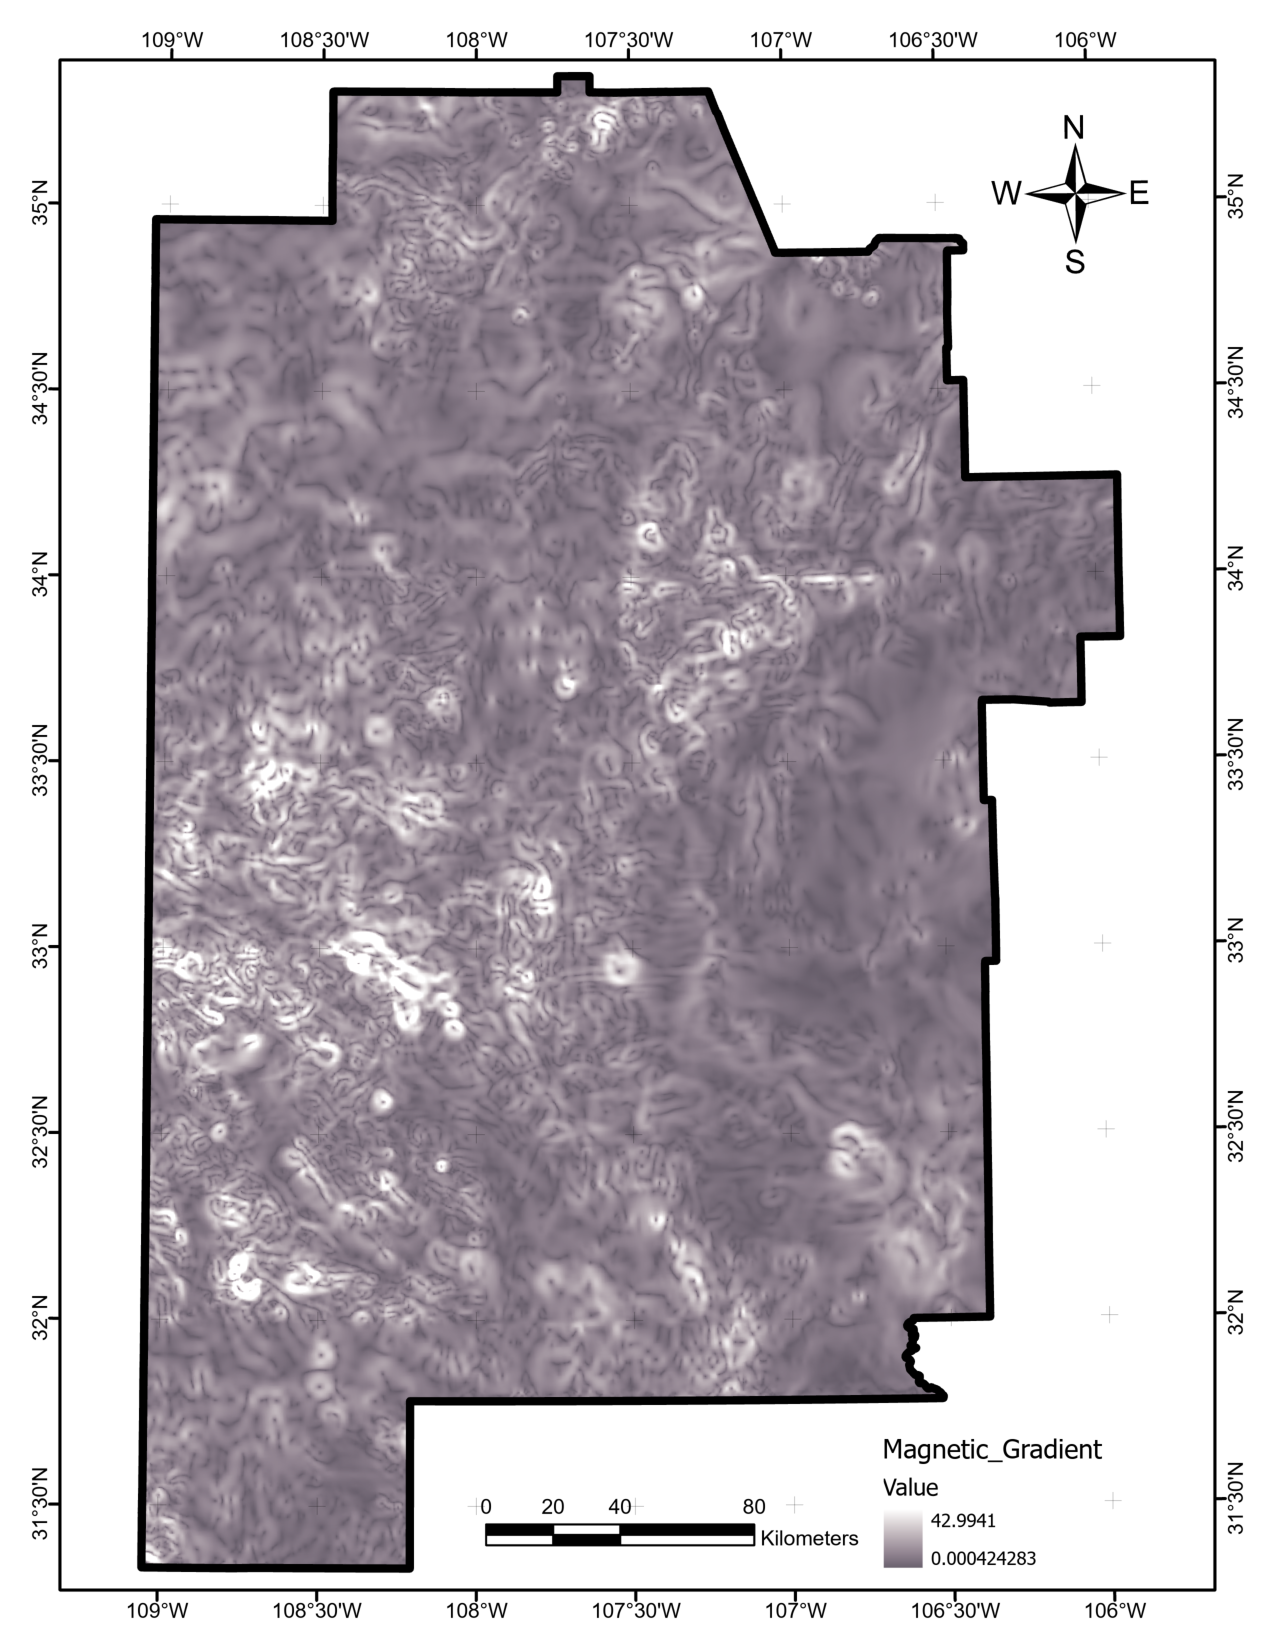
\includegraphics[width=0.75\linewidth]{templates/images/Figure-MagneticGradient.pdf}
\caption[Magnetic anomaly gradient data layer]{Magnetic anomaly gradient data layer. Units are in nT/degrees.}
\label{fig:feat_magnetic_gradient}
\end{figure}
\pagebreak

\section{Quaternary Fault Density}\label{app:dl_quat_fault_density}
Faults showing Quaternary displacement were digitized at the 1:24,000 scale by the New Mexico Bureau of Geology and Mineral Resources and provided to \citet{bielicki_hydrogeolgic_2015} and \citet{pepin_new_2019} in support of their investigations. The associated polyline features were downloaded from the PFA OpenEI submission \citep{kelley_geothermal_2015} and loaded into ArcGIS. As discussed for the Drainage Density layer, a Python-based kernel density workflow using extracted points from these polylines failed to produce satisfactory results. Instead, the ArcGIS \textit{Kernel Density} function was applied to create the final layer map (Figure \ref{fig:feat_qfaults}). Selected parameters for this function include an output cell size of 0.0025 degrees and auto-determined search radius of 0.367.
\vfill
\pagebreak

\begin{figure}[H]
\centering
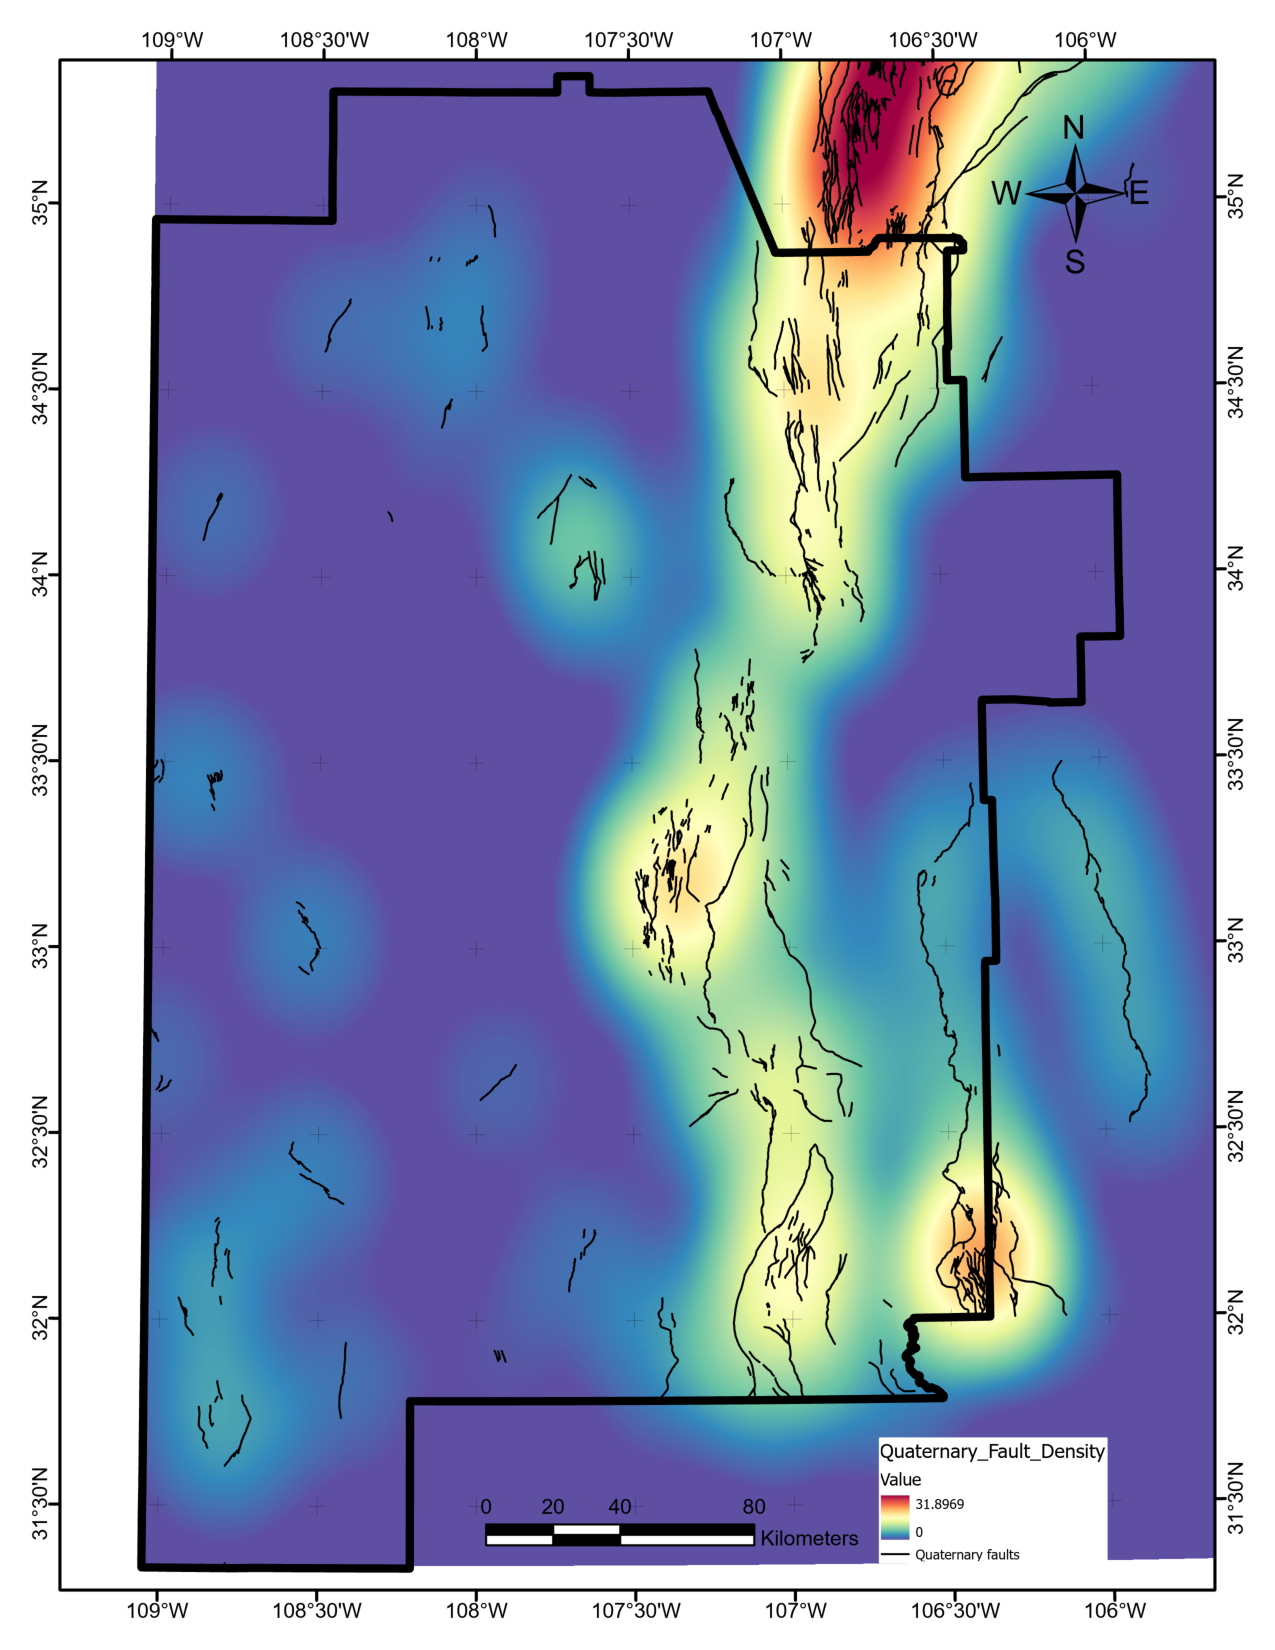
\includegraphics[width=0.75\linewidth]{templates/images/Figure-QFaultDensity.pdf}
\caption[Quaternary fault density data layer]{Quaternary fault density data layer. Units are in degrees/degrees$^2$. Black lines show the fault polyline data set archived by \protect\citet{bielicki_hydrogeolgic_2015}.}
\label{fig:feat_qfaults}
\end{figure}
\pagebreak

\section{Silica Geothermometer Temperature}\label{app:dl_geothermometer}
Silica concentration data from across the study area were compiled by \citet{bielicki_hydrogeolgic_2015}, and converted to reservoir temperatures using the Fournier chalcedony geothermometer relationship \citep{fournier_chemical_1977}. These data were downloaded from the Southwestern NM PFA OpenEI submission \citep{kelley_geothermal_2015} and merged together using ArcGIS and Python to create a single dataframe of 7,259 measurements, all within the broader Regional Polygon bounds to avoid surface creation edge effects within the tighter AOI. As described for the Boron Concentration data layer, attempts to model Si geothermometer estimates using Gaussian Processes provided unsatisfactory results. Instead, the final layer was created using the ArcGIS \textit{Empirical Bayes Kriging} routine. Selected parameters include: empirical data transformation type, a maximum of 100 points in each local model, 100 simulated semivariograms with k-Bessel model type, a standard circular search neighborhood with a radius of 1.196 (auto-determined), minimum of 10 neighbors, and maximum of 15 neighbors. The output grid cell size was set to 0.01 degrees. All coincident data were included in the calculation, so any overlapping measurements were considered in generating the final layer (Figure \ref{fig:feat_si_temp}).
\vfill
\pagebreak

\begin{figure}[H]
\centering
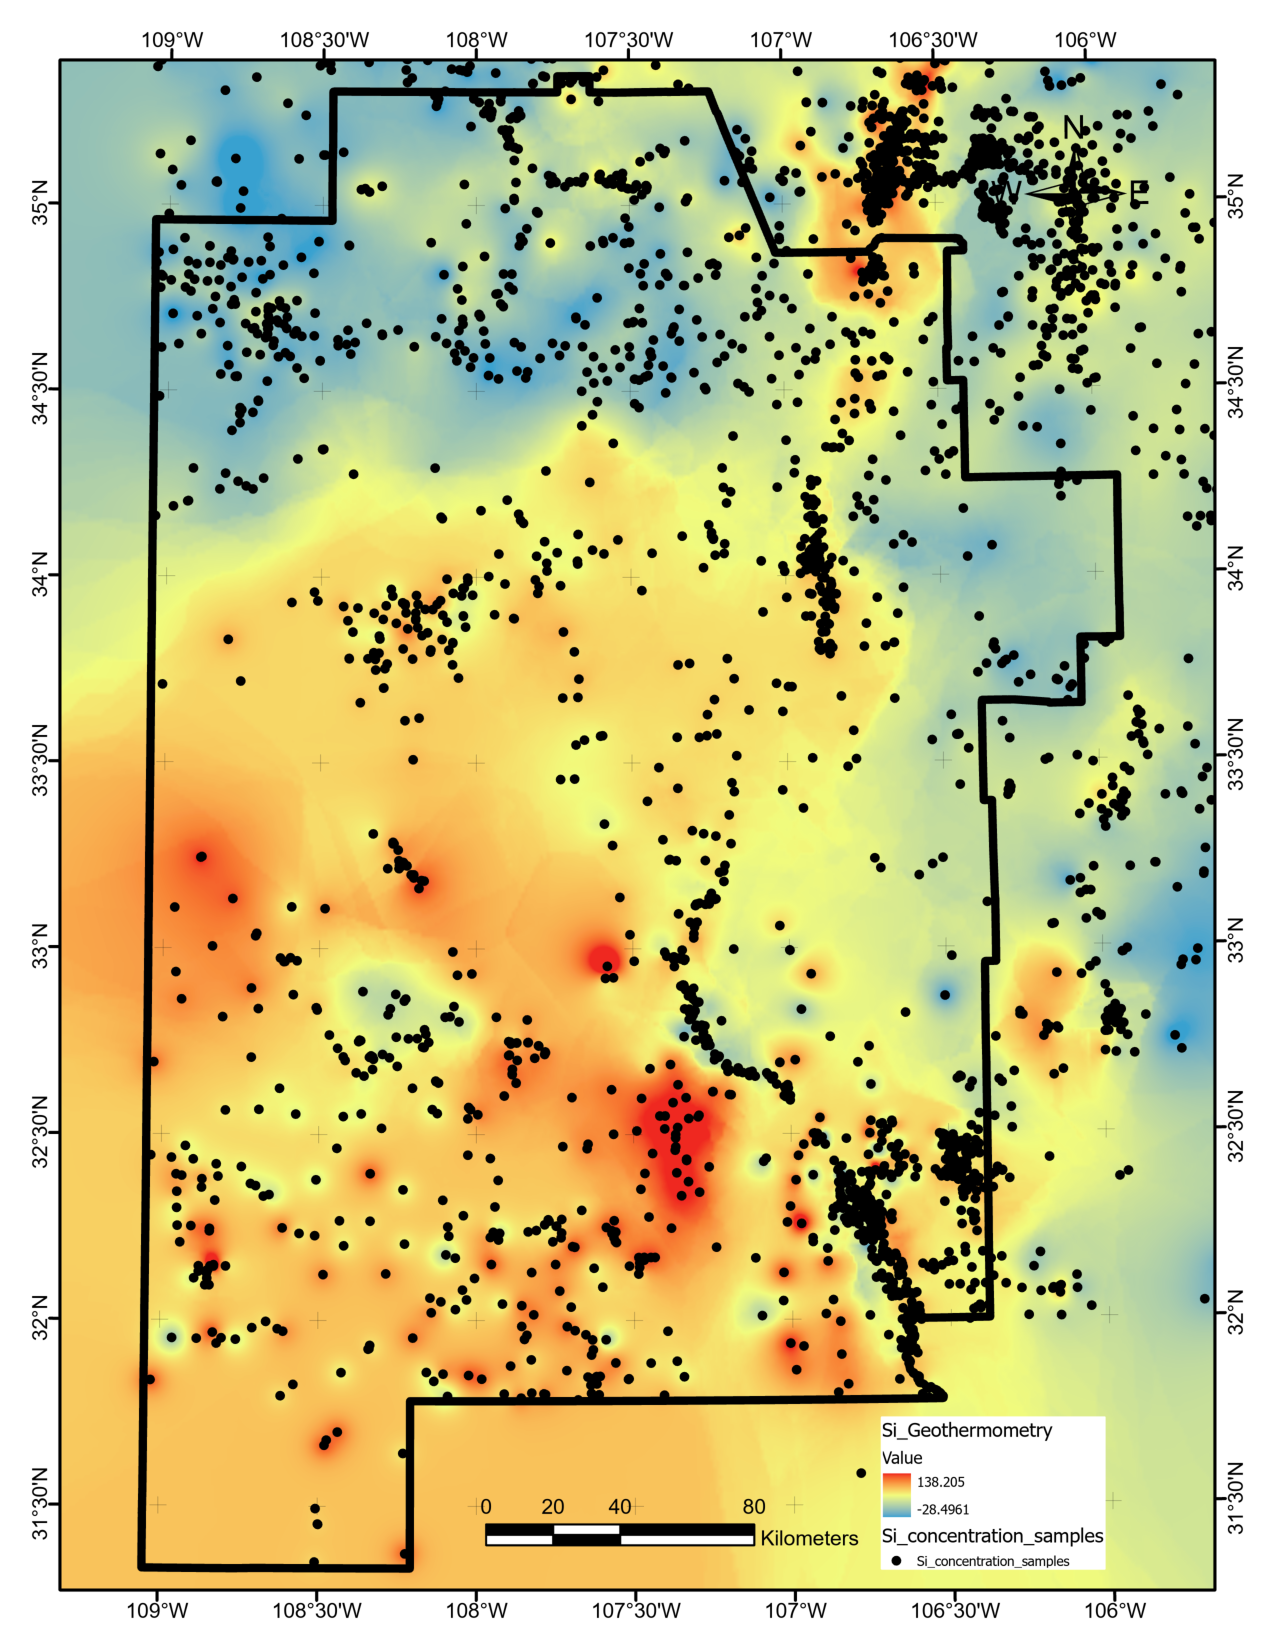
\includegraphics[width=0.75\linewidth]{templates/images/Figure-SiTemp.pdf}
\caption[Silica geothermometer temperature data layer]{Chalcedony geothermometer data layer. Units are in $^\circ$C. Black dots indicate locations where silica concentration was sampled, as collected by \protect\citet{bielicki_hydrogeolgic_2015}.}
\label{fig:feat_si_temp}
\end{figure}
\pagebreak

\section{Spring Density}\label{app:dl_spring_density}
The locations of springs in the study area were downloaded from the USGS National Water Information System \citep{usgs_national_2021}. A total of 2,565 springs were recorded within the bounds of the Regional Polygon. As with the Earthquake Density layer, this point set was loaded into a KDE Python script, which used a grid search routine to determine the best kernel radius for a Gaussian kernel density operator. Ten-fold cross validation identified the best radius value of 31,400 m (Figure \ref{fig:spring_cv}). 

\begin{figure}[H]
\centering
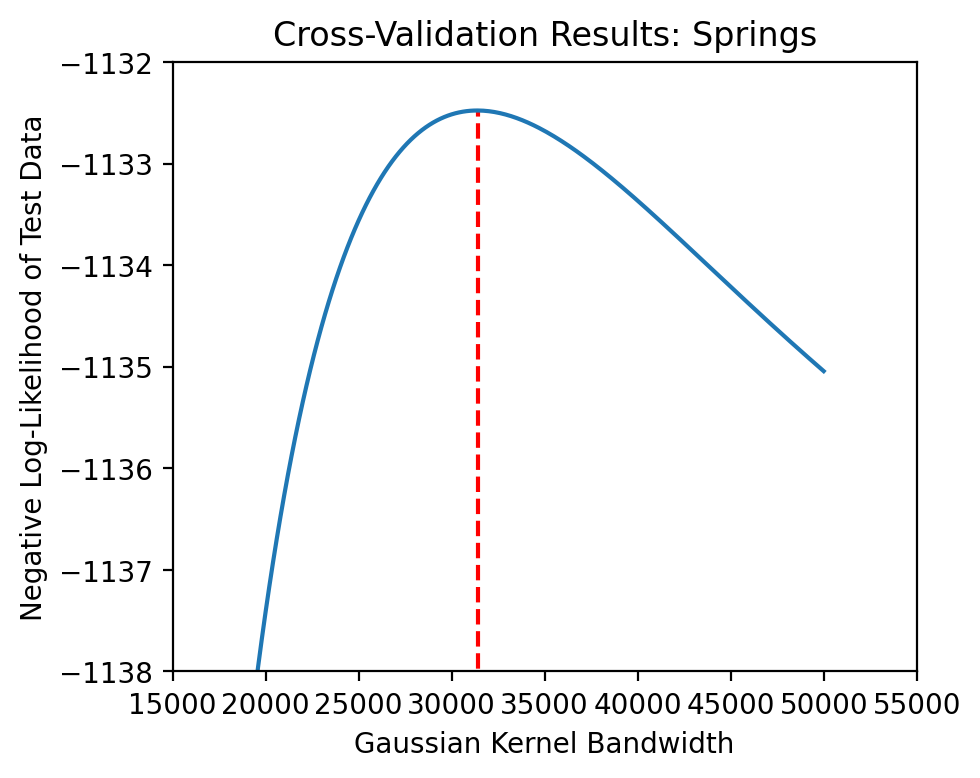
\includegraphics[scale=.60]{templates/images/Figure-Springs_kde_gridsearchcv_result.png}
\singlespacing
\caption[Spring density parameter tuning]{Cross-validation results for the springs KDE. Red dashed line indicates maximum negative log likelihood value identifying the best kernel radius.}
\label{fig:spring_cv}
\end{figure}

KDE values determined at each AOI mesh grid point location were loaded into ArcGIS, and \textit{Kriging} was used to generate a final layer for plotting purposes (Figure \ref{fig:feat_spring}). Selected \textit{Kriging} parameters included a spherical semivariogram model, lag size of 1e-6, variable search radius with 12-point requirement, and output cell size of 0.01.
\vfill
\pagebreak

\begin{figure}[H]
\centering
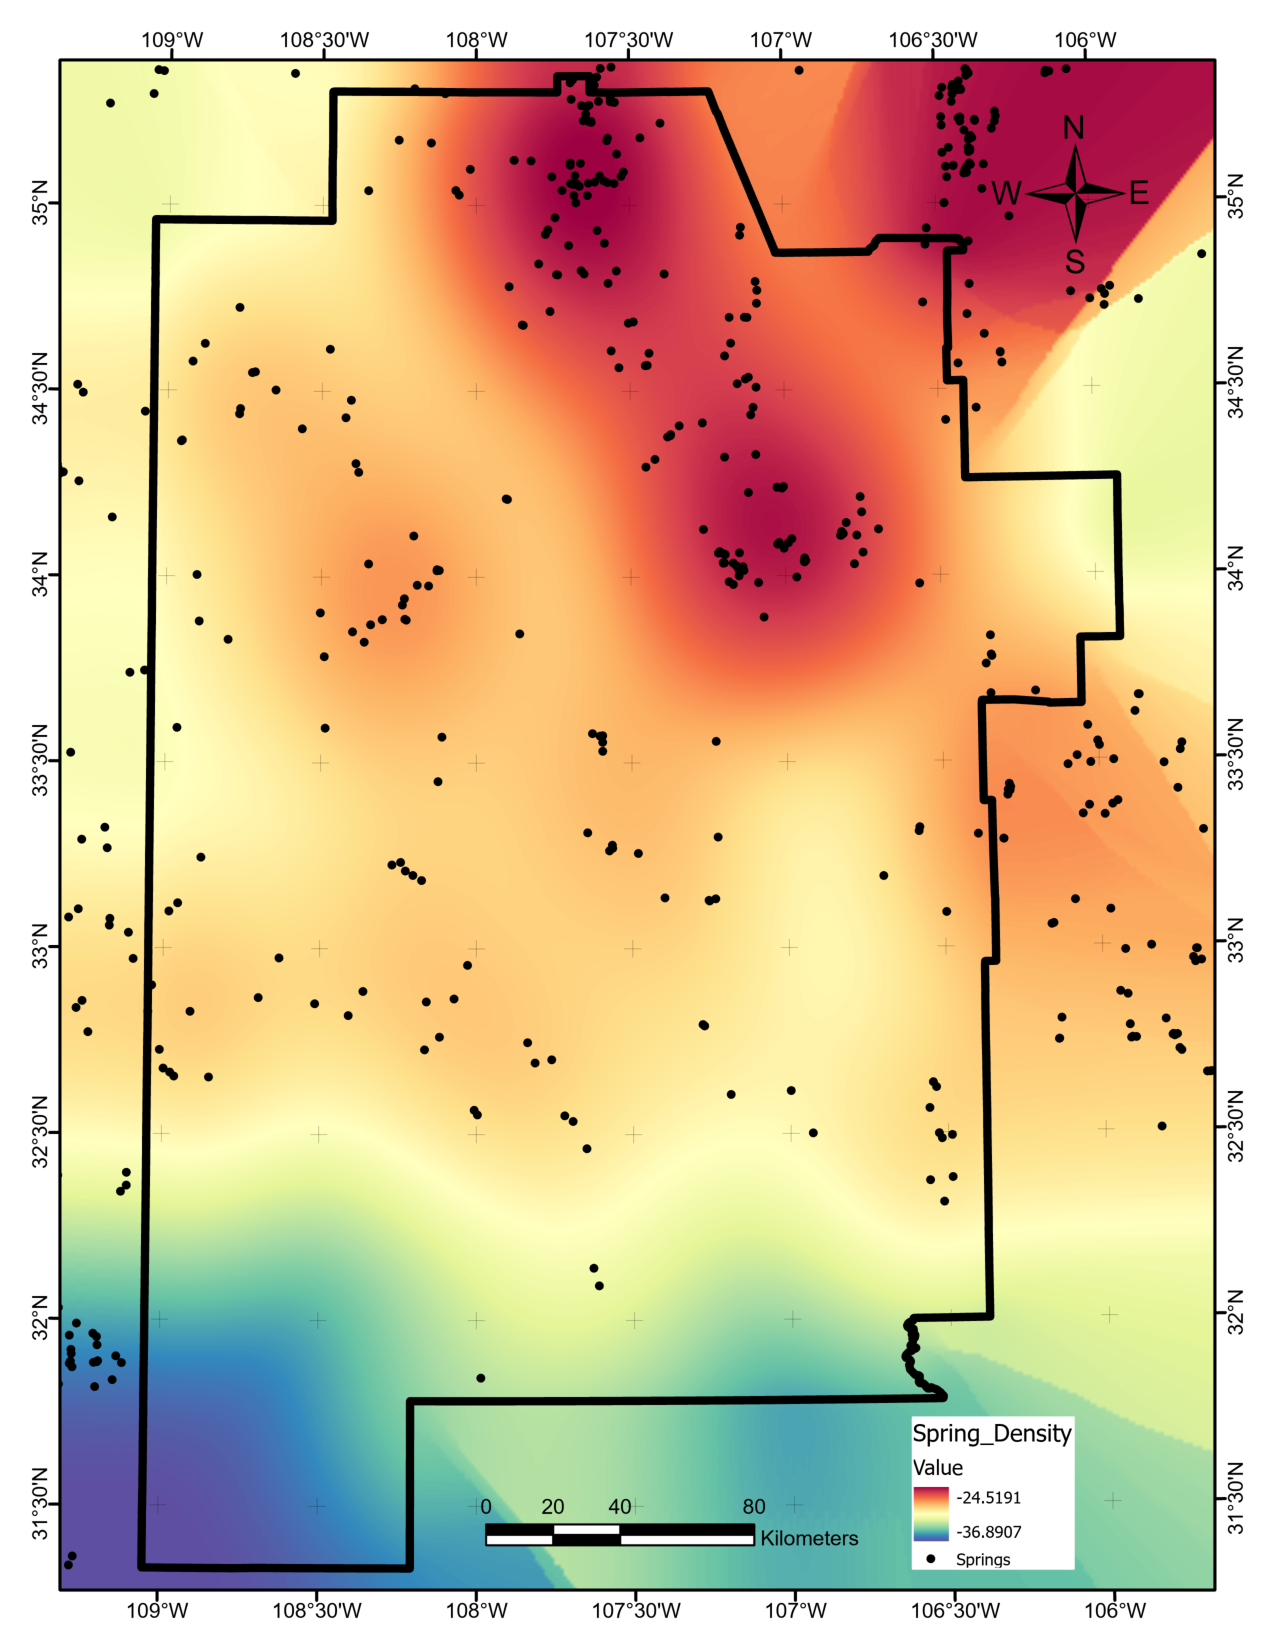
\includegraphics[width=0.75\linewidth]{templates/images/Figure-SpringDensity.pdf}
\caption[Spring density data layer]{Spring density data layer. Units are in log(points/km$^2$). Black dots indicate spring locations from the \protect\citet{usgs_national_2021}.}
\label{fig:feat_spring}
\end{figure}
\pagebreak

\section{State Map Fault Density}\label{app:dl_state_fault_density}
Digitized fault outlines from state geologic maps are available for download from the USGS Energy and Environment in the Rocky Mountain Area data portal \citep{usgs_eerma_2021}, including New Mexico state faults \citep{stoeser_usgs_2005}. These fault polylines were loaded into ArcGIS and, like the Quaternary faults, converted to fault density using the \textit{Kernel Density} operation (Figure \ref{fig:state_faults}). Selected parameters for this function include an output cell size of 0.0025 degrees and an auto-determined search radius of 0.252.
\vfill
\pagebreak

\begin{figure}[H]
\centering
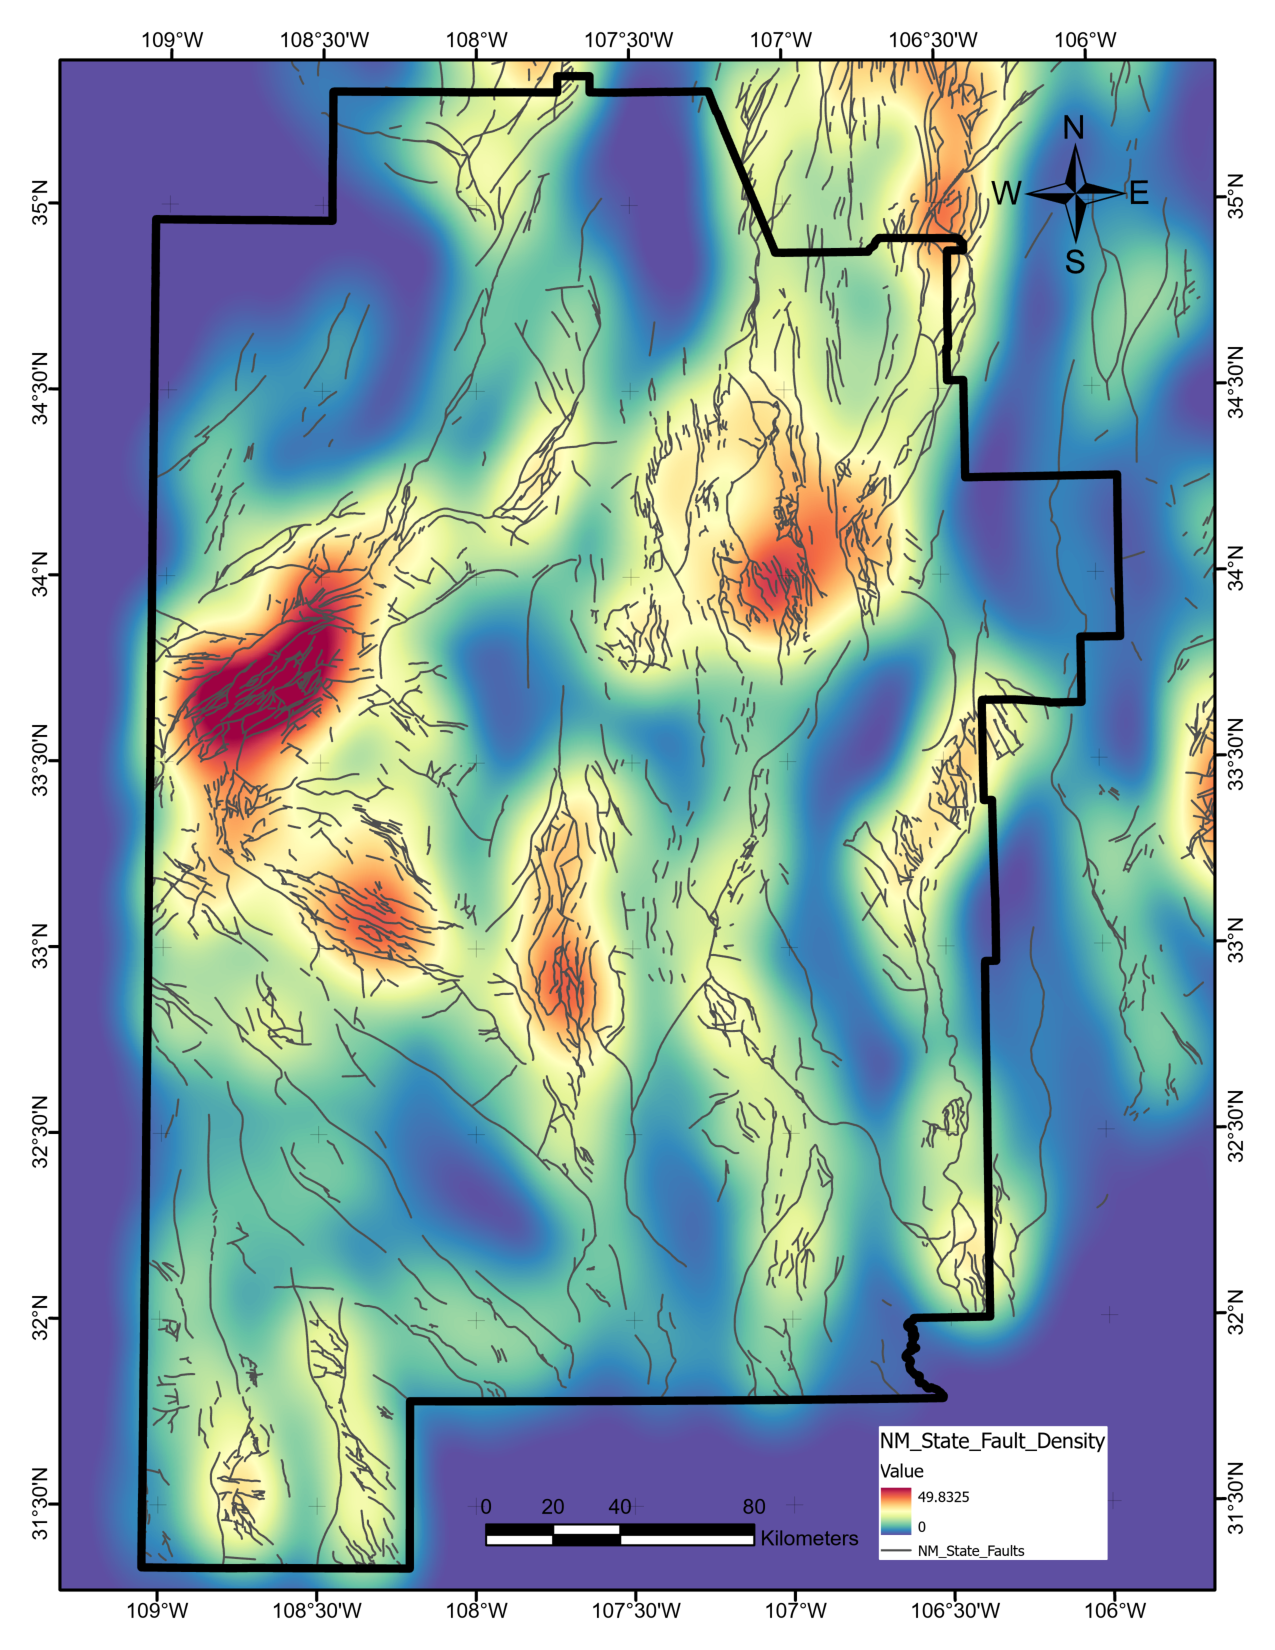
\includegraphics[width=0.75\linewidth]{templates/images/Figure-StateFaultDensity.pdf}
\caption[State fault density data layer]{State fault density data layer. Units are in degrees/degrees$^2$. Dark gray lines trace the fault polyline data set obtained from USGS Open-File Report 2005-1351 \protect\citep{stoeser_usgs_2005}.}
\label{fig:state_faults}
\end{figure}
\pagebreak

\section{Surface Topography (DEM)}\label{app:dl_dem}
The Southwestern NM PFA data archive \citep{kelley_geothermal_2015} includes a Digital Elevation Model (DEM) layer with surface elevations at a 1 arc-sec resolution. This layer was downloaded and imported into ArcGIS, however a data gap along the easternmost section of the AOI required the addition of two \(1^\circ\times1^\circ\) DEM tiles at the same resolution to fully complete the layer. These tiles were downloaded from the USGS National Map website \citep{usgs_tnm_2021} and merged with the original DEM. The final layer required no further processing (Figure \ref{fig:feat_dem}).
\vfill
\pagebreak

\begin{figure}[H]
\centering
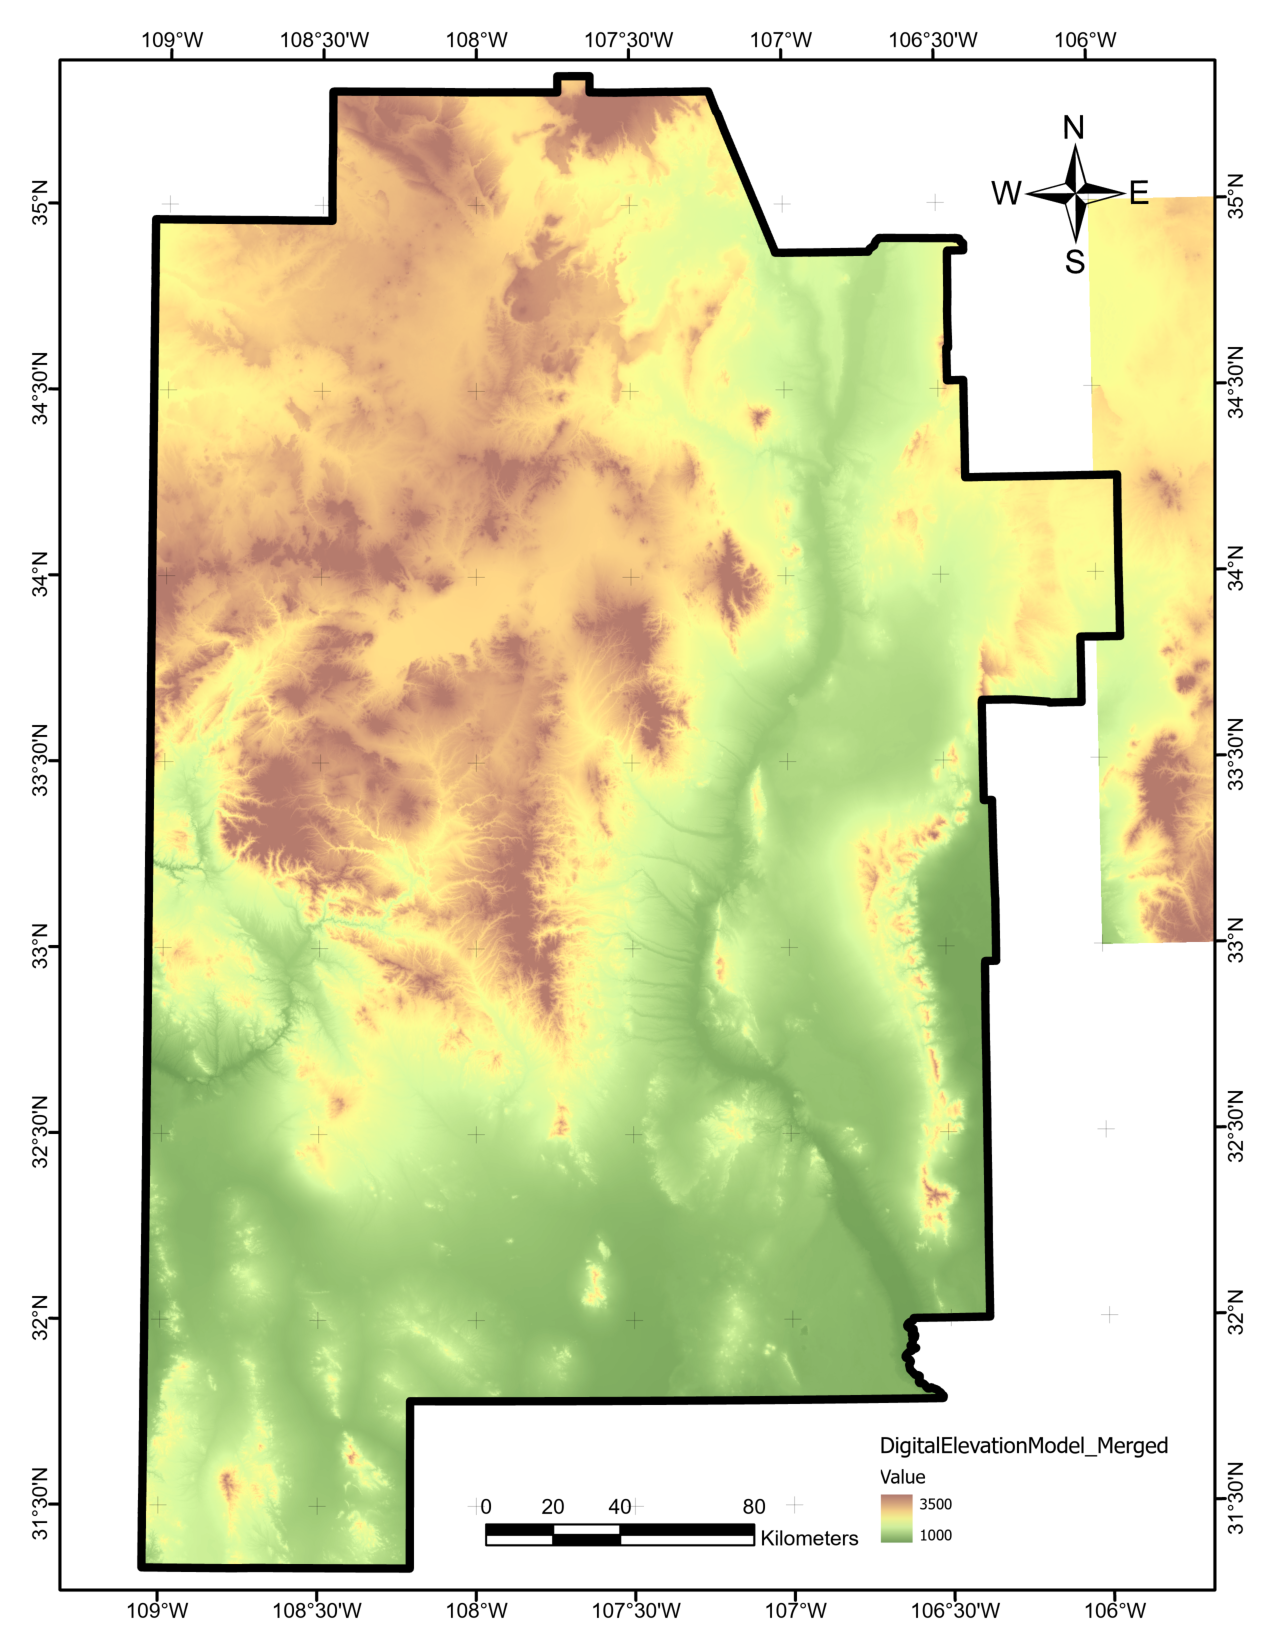
\includegraphics[width=0.8\textwidth]{templates/images/Figure-DEM.pdf}
\caption[Surface topography (DEM) data layer]{Surface topography (DEM) data layer. Units are in meters. Layer combines the DEM raster from \citet{bielicki_hydrogeolgic_2015} with data from The National Map online \citep{usgs_tnm_2021}.}
\label{fig:feat_dem}
\end{figure}
\pagebreak

\section{Topographic Gradient}\label{app:dl_dem_gradient}
Topographic gradient was calculated using the ArcGIS \textit{Slope} function on the final DEM layer. Parameters selected to create this layer include: geodesic method, z unit of meters, and output measurement of degrees (Figure \ref{fig:feat_dem_gradient}).

\begin{figure}[H]
\centering
\includegraphics[width=0.75\linewidth]{templates/images/Figure-DEMGradient.pdf}
\caption[Topographic gradient data layer]{Topographic gradient data layer. Units are in meters/degrees.}
\label{fig:feat_dem_gradient}
\end{figure}
\pagebreak

\section{Volcanic Dike Density}\label{app:dl_dike_density}
The USGS Energy and Environment in the Rocky Mountain Area data portal \citep{usgs_eerma_2021} also includes digitized volcanic dike outlines from the New Mexico state geologic map \citep{stoeser_usgs_2005}. These polylines were imported into ArcGIS and, like the Quaternary fault data set, converted to density using the \textit{Kernel Density} operation (Figure \ref{fig:feat_dikes}). Selected parameters for this function included an output cell size of 0.0025 degrees and an auto-determined search radius of 0.252.

\begin{figure}[H]
\centering
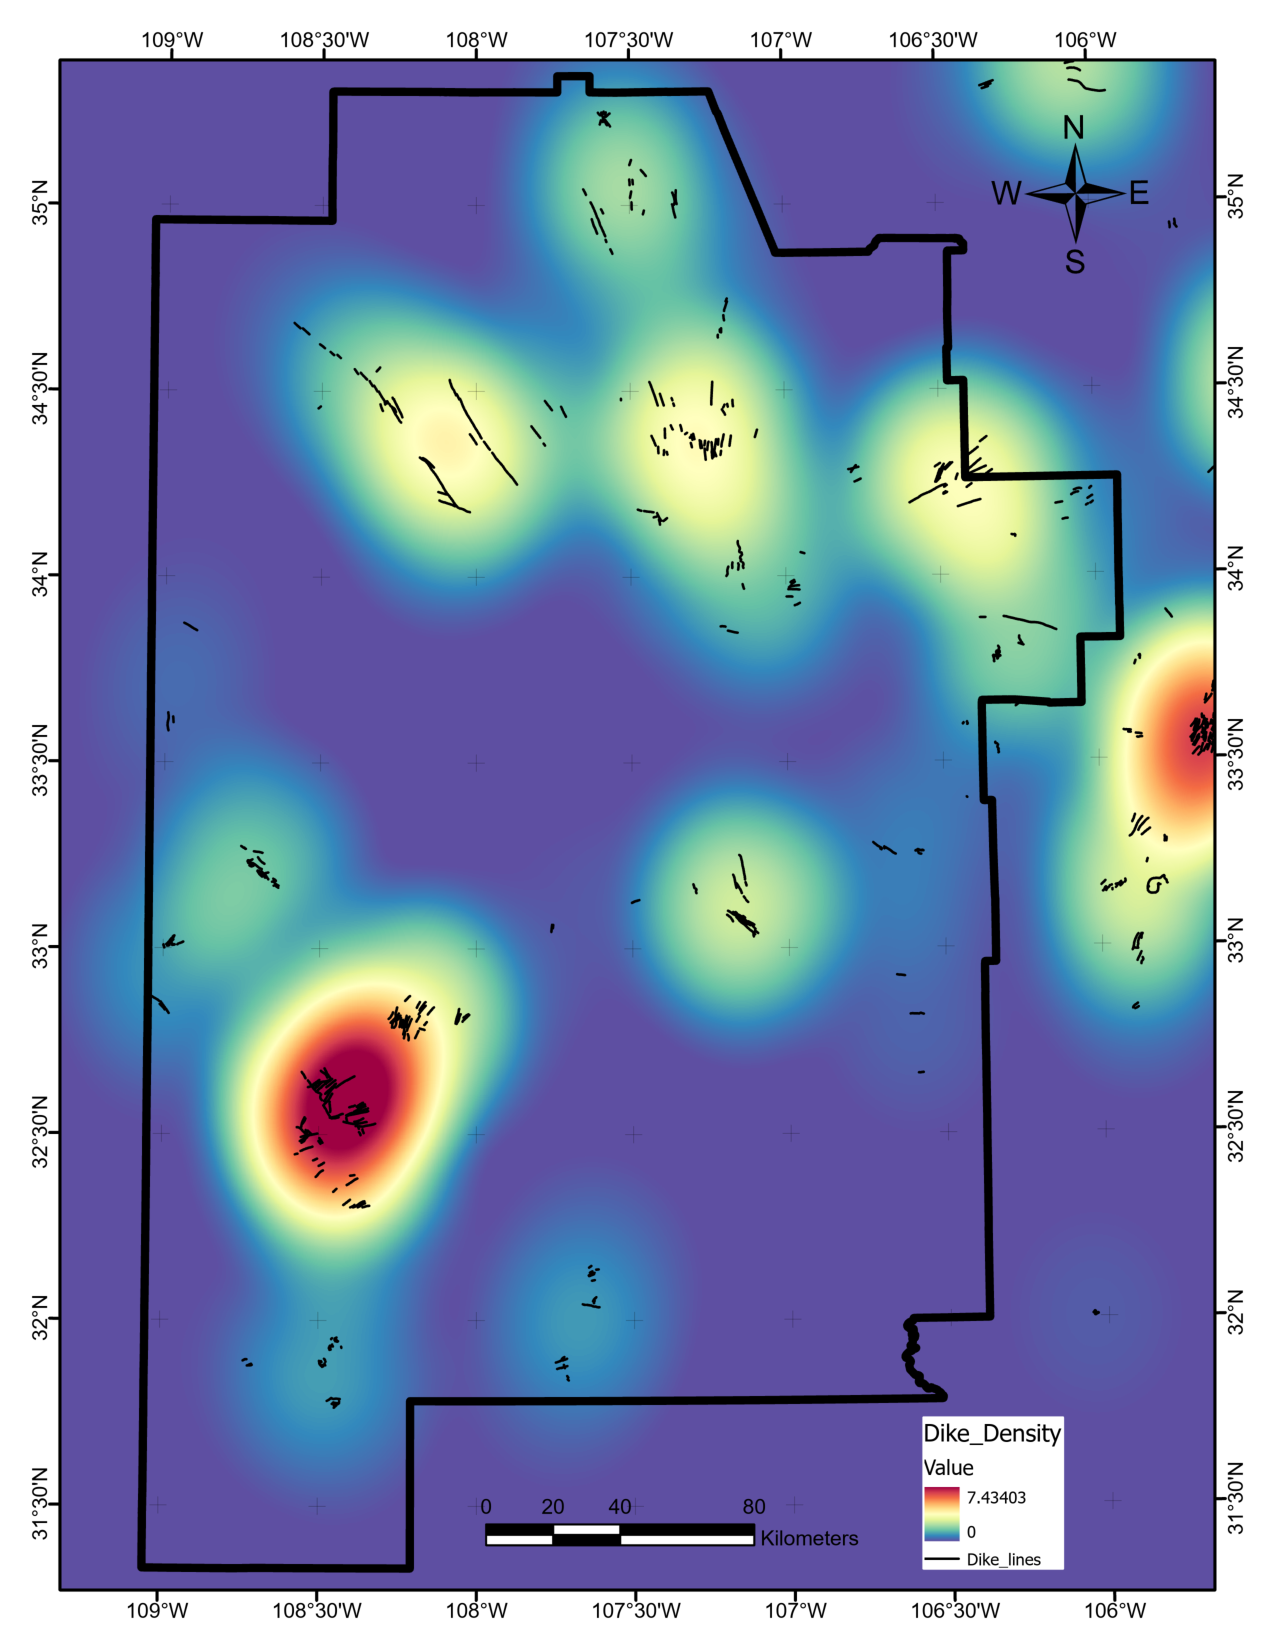
\includegraphics[width=0.75\linewidth]{templates/images/Figure-DikeDensity.pdf}
\caption[Volcanic dike data layer]{Volcanic dike density data layer. Units are in degrees/degrees$^2$. Black lines trace the dike polyline data set obtained from USGS Open-File Report 2005-1351 \protect\citep{stoeser_usgs_2005}}
\label{fig:feat_dikes}
\end{figure}
\pagebreak

\section{Volcanic Vent Density}\label{app:dl_vent_density}
Volcanic vents identified in the study area were retrieved from the New Mexico Bureau of Geology and Mineral Resources using the NMBGMR Interactive Map \citep{nmbgmr_nmbgmr_2021}. A total of 811 volcanic vents are observed within the geographic bounds of the Regional Polygon. As with the Earthquake Density layer, the point set was loaded into a KDE Python script, which used a grid search routine to determine the optimal kernel radius. Ten-fold cross validation suggested a radius of 28,300 m (Figure \ref{fig:vent_cv}).

\begin{figure}[H]
\centering
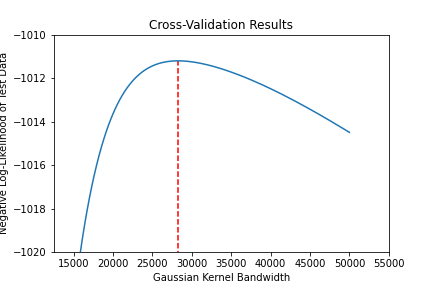
\includegraphics[scale=.60]{templates/images/Figure-Vents_kde_gridsearchcv_result.png}
\caption[Volcanic vent density parameter tuning]{Cross-validation results for volcanic vent KDE. Red dashed line indicates maximum negative log likelihood value identifying the best kernel radius.}
\label{fig:vent_cv}
\end{figure}

KDE values calculated at each AOI mesh grid point location were loaded into ArcGIS, and \textit{Kriging} was used to generate a final layer for plotting purposes (Figure \ref{fig:feat_vents}). \textit{Kriging} parameters included spherical semivariogram model, lag size of 1e-6, variable search radius with 12-point requirement, and output cell size of 0.01. 
\vfill
\pagebreak

\begin{figure}[H]
\centering
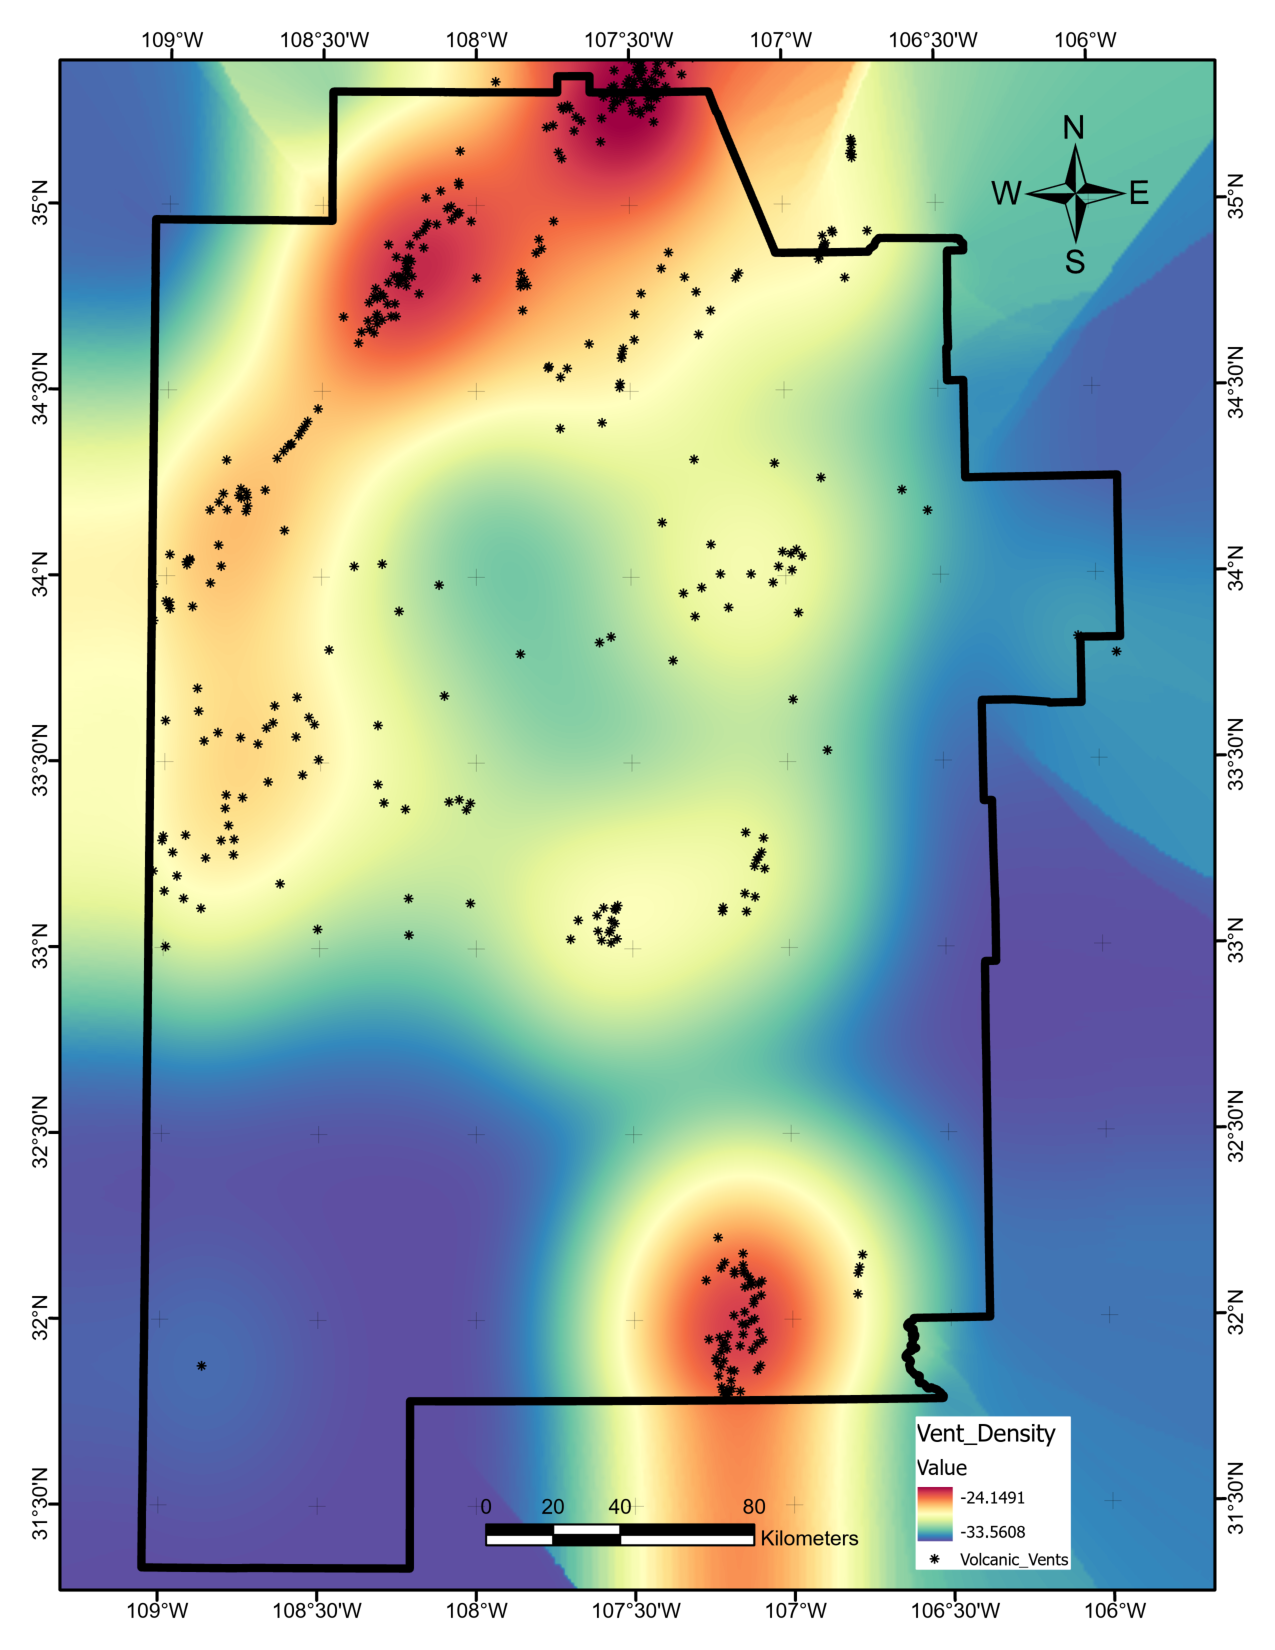
\includegraphics[width=0.75\linewidth]{templates/images/Figure-VentDensity.pdf}
\caption[Volcanic vent data layer]{Volcanic vent density data layer. Units are in log(points/km$^2$). Black dots indicate vent locations from the \protect\citet{nmbgmr_nmbgmr_2021}}
\label{fig:feat_vents}
\end{figure}
\pagebreak

\section{Water Table Depth}\label{app:dl_wt_depth}
\citet{bielicki_hydrogeolgic_2015} mapped depth to the water table using data from the USGS and several additional sources. This raster was downloaded from their OpenEI submission \citep{kelley_geothermal_2015} and imported into ArcGIS. Data gaps between the raster extent and AOI polygon to the south and the east necessitated extrapolation of the layer, so ArcGIS \textit{Empirical Bayes Kriging} was applied to fill in the missing values. After some trial-and-error, the chosen parameter values included: output cell size of 0.01, empirical data transformation type, maximum of 100 points in each local model, 100 simulated exponential semivariograms, a standard circular search neighborhood with a radius of 1.265 (auto-determined), minimum of 10 neighbors, and maximum of 15 neighbors. Figure \ref{fig:feat_wtdepth} shows the final layer.
\vfill
\pagebreak

\begin{figure}[H]
\centering
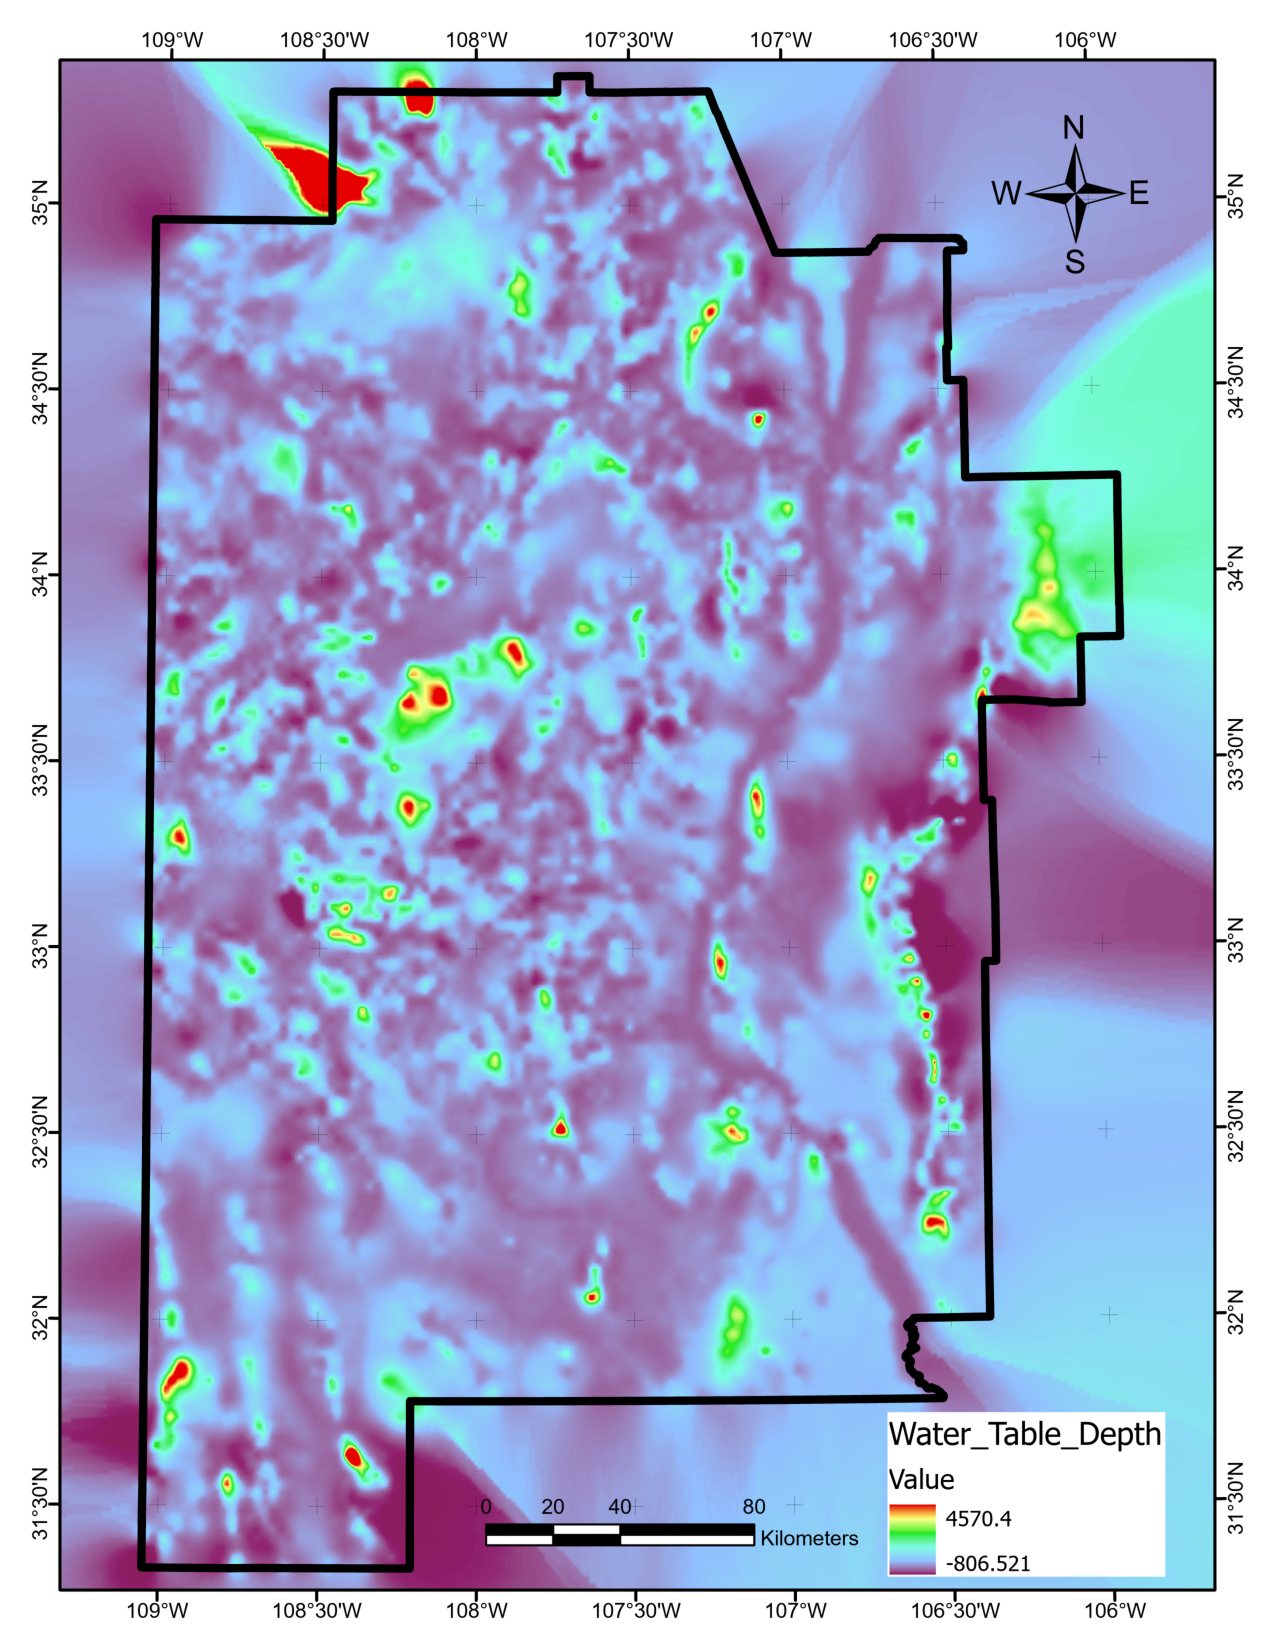
\includegraphics[width=0.75\linewidth]{templates/images/Figure-WTDepth.pdf}
\caption[Water table depth data layer]{Water table depth data layer. Units are in feet. Adapted from raster created by \protect\citep{bielicki_hydrogeolgic_2015}.}
\label{fig:feat_wtdepth}
\end{figure}
\pagebreak

\section{Water Table Gradient}\label{app:dl_wt_gradient}
A pre-calculated grid for the water table gradient is among the layers included in the Southwestern NM PFA archive \citep{kelley_geothermal_2015}. This raster was downloaded and imported into ArcGIS. In order to fill data gaps between the raster extent and the AOI polygon to the south and the east, the ArcGIS \textit{Empirical Bayes Kriging} process was applied. After some trial-and-error, the final layer was generated using the following parameter values: output cell size of 0.01, empirical data transformation type, maximum of 100 points in each local model, 100 simulated exponential semivariograms, a standard circular search neighborhood with a radius of 1.265 (auto-determined), minimum of 10 neighbors, and maximum of 15 neighbors (Figure \ref{fig:feat_wt_gradient}).
\vfill
\pagebreak

\begin{figure}[H]
\centering
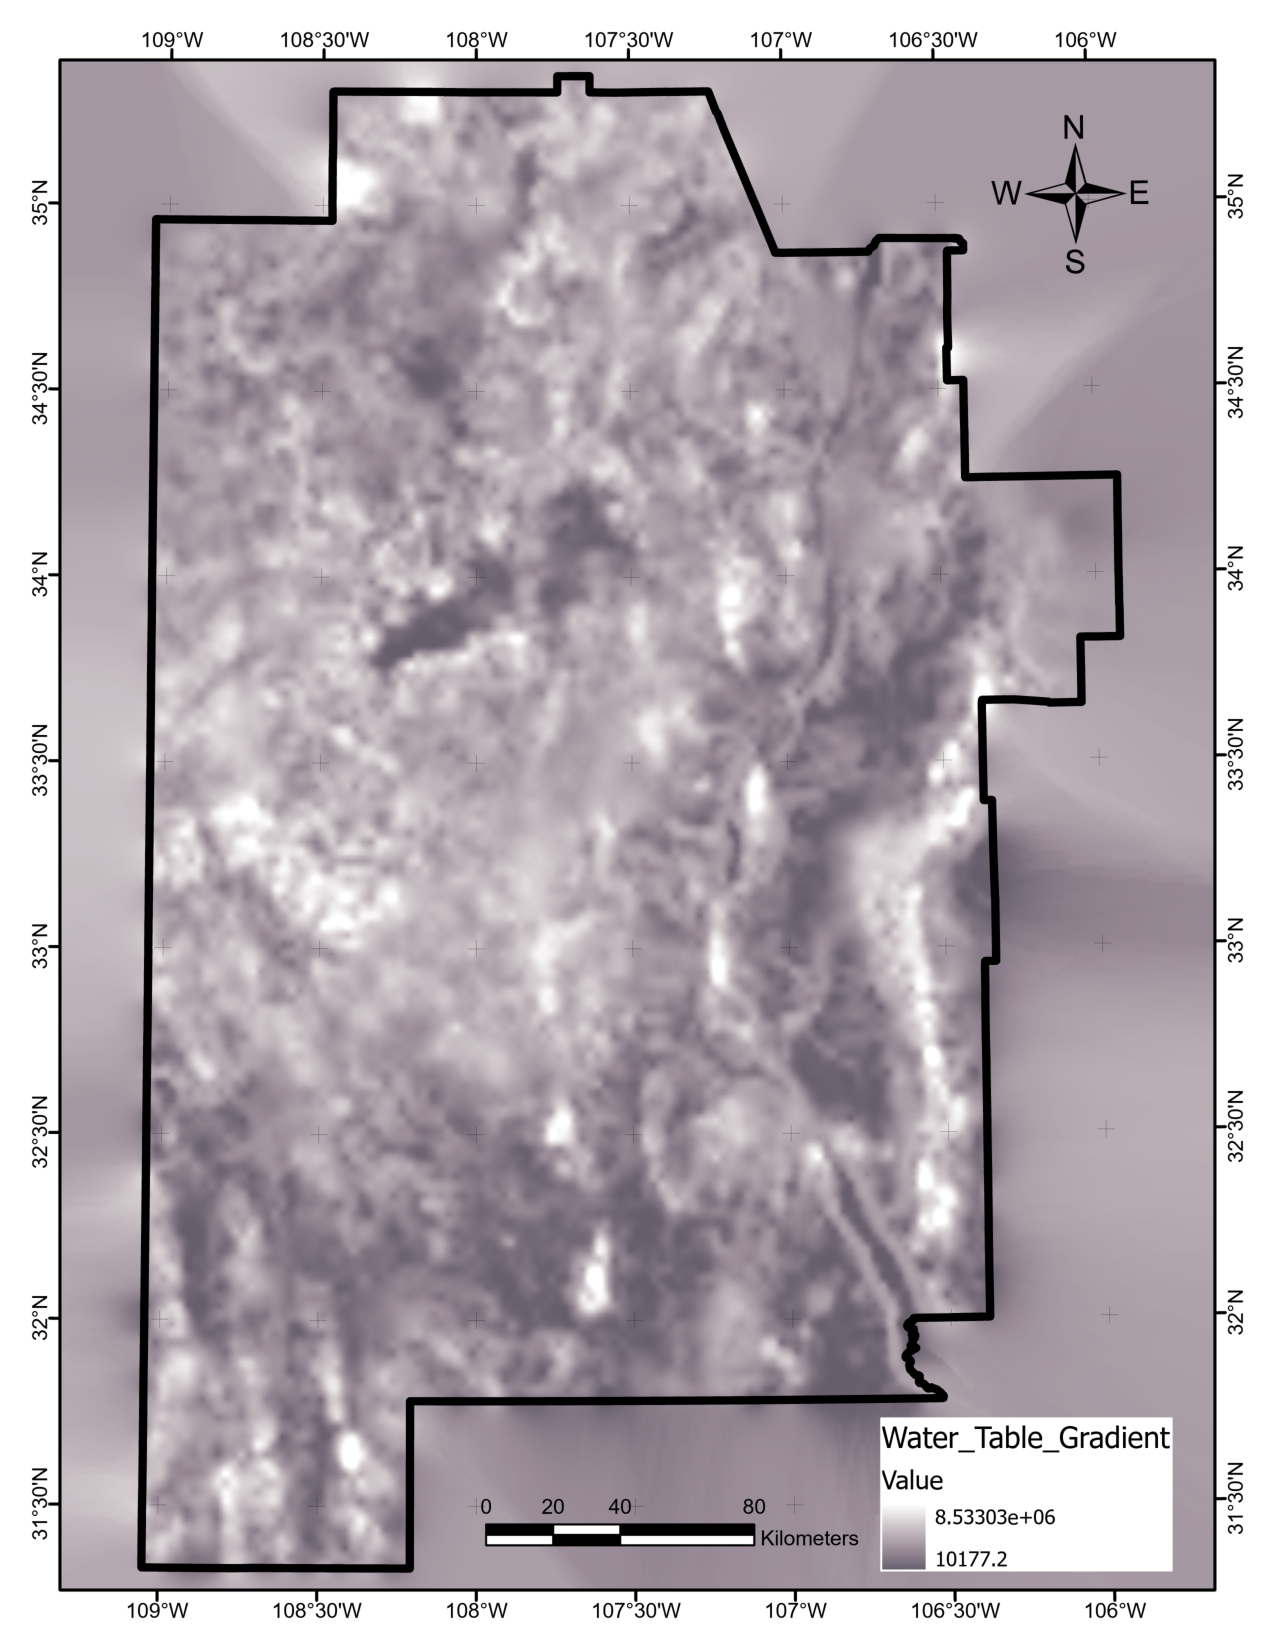
\includegraphics[width=0.75\linewidth]{templates/images/Figure-WTGradient.pdf}
\caption[Water table gradient data layer]{Water table gradient data layer. Units are in feet/degrees. Based on the raster from \protect\citet{bielicki_hydrogeolgic_2015}.}
\label{fig:feat_wt_gradient}
\end{figure}
\pagebreak

\section{Geothermal Gradient}\label{app:dl_geothermal_gradient}
The response variable for this analysis comes from observations stored in the SMU \textit{Heat Flow Database from Bottom Hole Temperature Data}, accessed via the SMU node of the \acrlong{ngds} \citep{smu_geothermal_2021}. This database focuses specifically on heat flow values derived using geothermal gradient and conductivity measurements from well data in journal articles, books, reports, and from other sources \citep{blackwell_geothermal_2014}. Geothermal gradient values are provided in two forms: reported gradient and corrected gradient. The latter reports the result of both temperature and terrain corrections based on the well depth interval that a measurement was taken. If a corrected geothermal gradient value existed, this value was used in this analysis, otherwise the regular geothermal gradient value was selected. The well data set was clipped to the bounds of the Regional Polygon, then loaded into Python for conditioning. Well records missing geographic coordinates or a geothermal gradient value of either type were dropped. The list was sorted on coordinates and gradient, and only the first record for each location was kept. The sort was in descending order, so this method preserved the highest gradient value captured per well. The final set of 596 values shown in Figure \ref{fig:feat_geotherm_gradient} comprise the raw input data used for predictive modeling of geothermal gradient across the study AOI.
\vfill
\pagebreak

\begin{figure}[H]
\centering
\includegraphics[width=0.75\linewidth]{templates/images/Figure-GeothermalGrad_OrigWells.pdf}
\caption[Geothermal gradient well data]{Geothermal gradient observations from well data. Units are in K/km. Data were retrieved from the SMU NGDS portal \protect\citep{smu_geothermal_2021}.}
\label{fig:feat_geotherm_gradient}
\end{figure}
\pagebreak

A geothermal gradient layer also exists within the \citeauthor{bielicki_hydrogeolgic_2015} OpenEI submission \citep{kelley_geothermal_2015}, based primarily on a prior version of the SMU well data set. The layer nearly covers the full AOI, except for a missing section in the southwestern ``boot-heel'' of the state (Figure \ref{fig:feat_pfa_geotherm_gradient}A). Extrapolation was performed using the ArcGIS \textit{Empirical Bayes Kriging} function to create a complete map using the following parameters: output cell size of 0.01, empirical data transformation type, a maximum of 100 points in each local model, 100 simulated semivariograms with exponential model type, a standard circular search neighborhood with a radius of 1.265 (auto-determined), minimum of 10 neighbors, and maximum of 15 neighbors. This layer was saved as a reference map for later comparison with predictive model results (Figure \ref{fig:feat_pfa_geotherm_gradient}B).  

\begin{figure}[H]
\centering
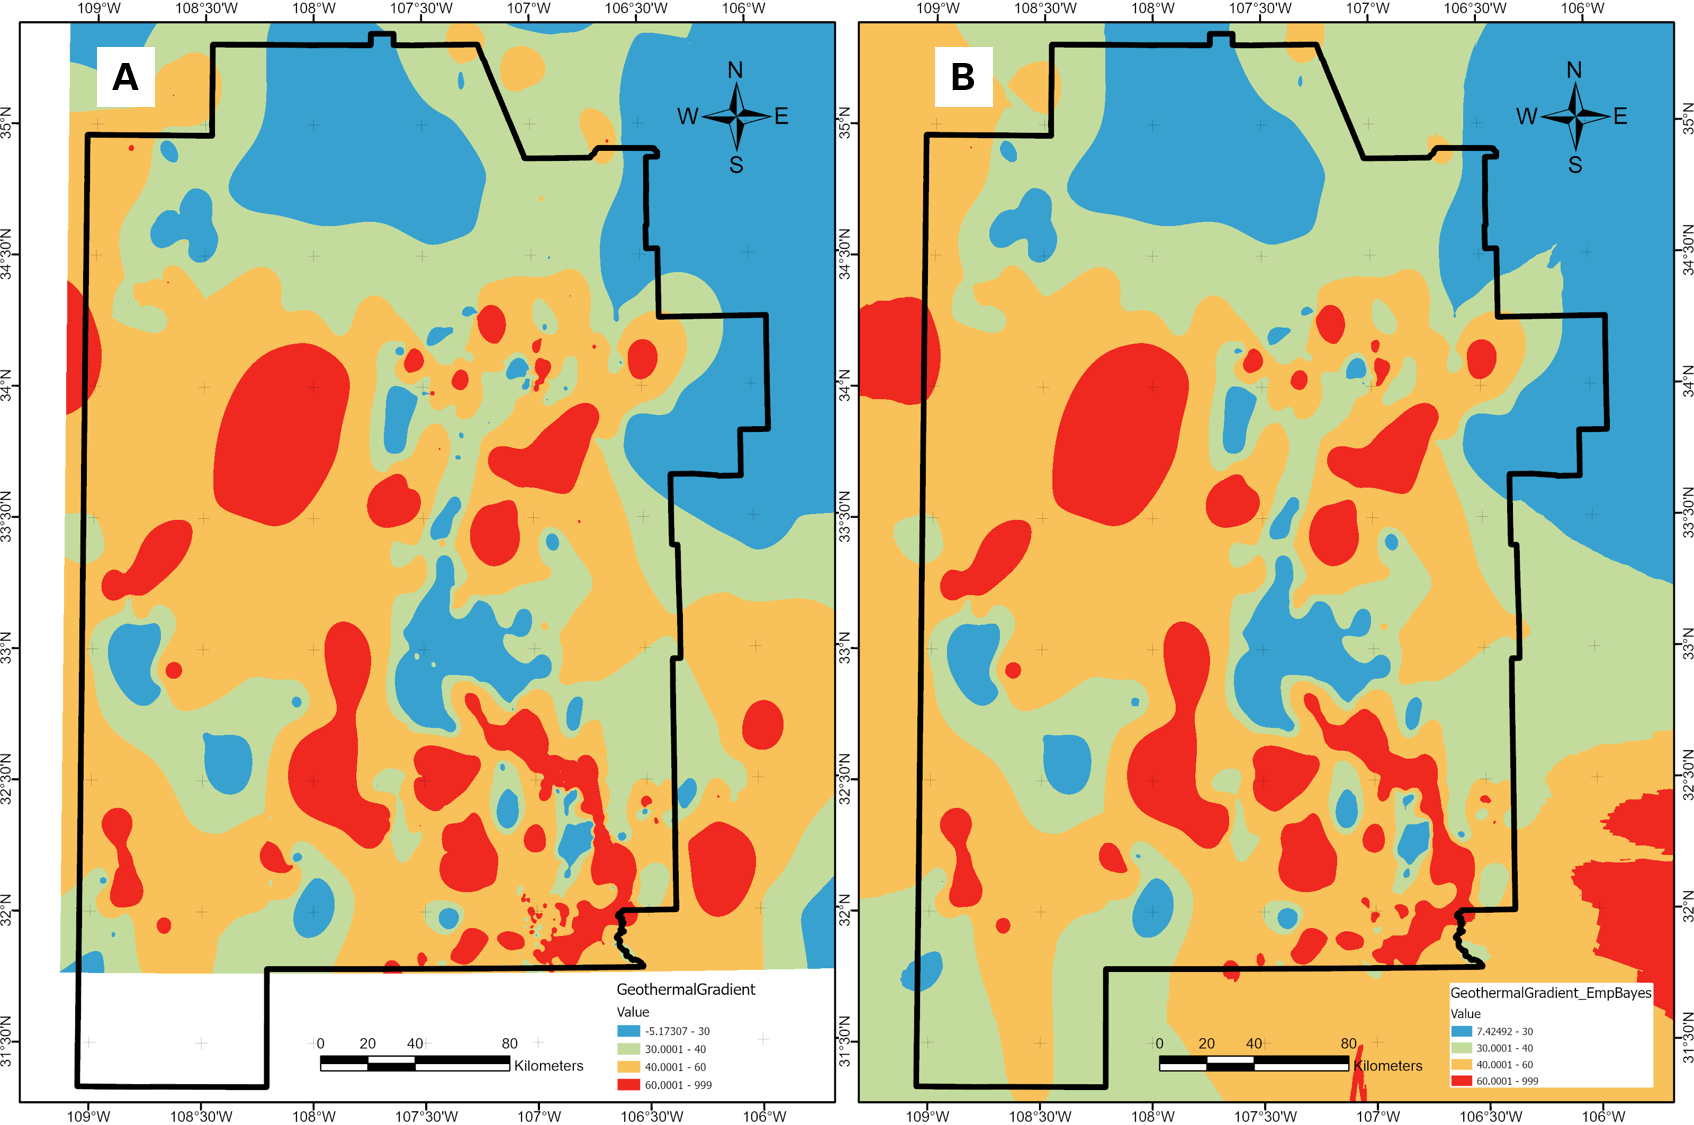
\includegraphics[width=\linewidth]{templates/images/Figure-PFA_Geothermal_Gradient_sidebyside.png}
\caption[Geothermal gradient data layer]{Geothermal gradient data layer. Units are in K/km. A. Raster originally created by \protect\citet{bielicki_hydrogeolgic_2015}. B. Extrapolation performed using the ArcGIS \textit{Empirical Bayes Kriging} to fill in the southwestern data gap.}
\label{fig:feat_pfa_geotherm_gradient}
\end{figure}
